\documentclass[12pt]{article}

\usepackage{answers}
\usepackage{setspace}
\usepackage{graphicx}
\usepackage{enumitem}
\usepackage{multicol}
\usepackage{mathrsfs}
\usepackage[margin=1in]{geometry} 
\usepackage{amsmath,amsthm,amssymb}
\usepackage[ngerman]{babel}

\newcommand{\N}{\mathbb{N}}
\newcommand{\Z}{\mathbb{Z}}
\newcommand{\C}{\mathbb{C}}
\newcommand{\R}{\mathbb{R}}

\DeclareMathOperator{\sech}{sech}
\DeclareMathOperator{\csch}{csch}

\newenvironment{theorem}[2][Theorem]{\begin{trivlist}
		\item[\hskip \labelsep {\bfseries #1}\hskip \labelsep {\bfseries #2.}]}{\end{trivlist}}
\newenvironment{definition}[2][Definition]{\begin{trivlist}
		\item[\hskip \labelsep {\bfseries #1}\hskip \labelsep {\bfseries #2.}]}{\end{trivlist}}
\newenvironment{proposition}[2][Proposition]{\begin{trivlist}
		\item[\hskip \labelsep {\bfseries #1}\hskip \labelsep {\bfseries #2.}]}{\end{trivlist}}
\newenvironment{lemma}[2][Lemma]{\begin{trivlist}
		\item[\hskip \labelsep {\bfseries #1}\hskip \labelsep {\bfseries #2.}]}{\end{trivlist}}
\newenvironment{exercise}[2][Exercise]{\begin{trivlist}
		\item[\hskip \labelsep {\bfseries #1}\hskip \labelsep {\bfseries #2.}]}{\end{trivlist}}
\newenvironment{solution}[2][Solution]{\begin{trivlist}
		\item[\hskip \labelsep {\bfseries #1}]}{\end{trivlist}}
\newenvironment{problem}[2][Problem]{\begin{trivlist}
		\item[\hskip \labelsep {\bfseries #1}\hskip \labelsep {\bfseries #2.}]}{\end{trivlist}}
\newenvironment{question}[2][Question]{\begin{trivlist}
		\item[\hskip \labelsep {\bfseries #1}\hskip \labelsep {\bfseries #2.}]}{\end{trivlist}}
\newenvironment{corollary}[2][Corollary]{\begin{trivlist}
		\item[\hskip \labelsep {\bfseries #1}\hskip \labelsep {\bfseries #2.}]}{\end{trivlist}}

\begin{document}
	\title{Machine Learning for Natural Language Processing}
	\author{Michael Gabler}
	\maketitle
	\tableofcontents
	\newpage

	\section{Grundlagen}
	Neuronales Netzwerk ist Funktion, die auf Eingabedaten angewendet wird.\\
	\textbf{Optimierung} durch Minimierung der Loss-Funktion\\
	\textbf{Loss-Funktion} Maß, wie gut das Netzwerk Vorhersagen trifft. Berechnet sich aus Vorhersage und tatsächlichen Werten (Ground Truth).
	\begin{itemize}
		\item Euklidischer Loss, Mean-Squared-Error: $l_2 = \frac{1}{2N} \sum_i (f_\theta(x_i)-t_i)^2$
		\item Negative-Log-Likelihood, Cross-Entropy: $NLL = -\frac{1}{|D|}\sum_i \log[f_\theta(x_i)|_{t_i}]$
	\end{itemize}
	\textbf{Konfusionsmatrix} welche Klassen werden wie oft mit welcher Klasse verwechselt?\\
	
	\subsection{Training}
	Daten werden aufgeteilt in Train/Validierung/Test (z.B. 60/20/20)\\
	\textbf{Datenaugmentierung} Generieren zusätzlicher Daten (z.B. bei Bildern) durch Spiegelung, Rotation, Skalierung, Anpassung Helligkeit und Farbe, etc.\\
	\textbf{Epoche} Verarbeitung aller Trainingsdaten\\
	\textbf{Iteration} Verarbeitung eines Batches\\
	\textbf{Batch} Mehrere Trainingsbeispiele werden gerechnet bevor Gewichte einmal geupdated werden (z.B. 10 Beispiele pro Batch)\\
	\textbf{Learning Rate} Faktor $\eta$, wie stark das Netzwerk durch die Deltas verändert werden soll (d.h. wie schnell es lernt bzw. seine Meinung ändert). Wird beim Update der Gewichte verwendet.
	\textbf{Evaluation auf Validierungsdaten} zur Anpassung der Hyperparameter (Learning-Rate, Netzstruktur, ...)\\
	\textbf{Evaluation auf Testdaten} einmalig, um Genauigkeit des trainierten Netzes zu ermitteln
	\textbf{Forward-Pass} Berechnen des Outputs des Netzwerkes für bestimmte Eingabedaten (z.B. ein Batch)\\
	\textbf{Backward-Pass} Bilden der partiellen Ableitung für jeden Input in jedem Layer und Speichern der Werte als Deltas\\
	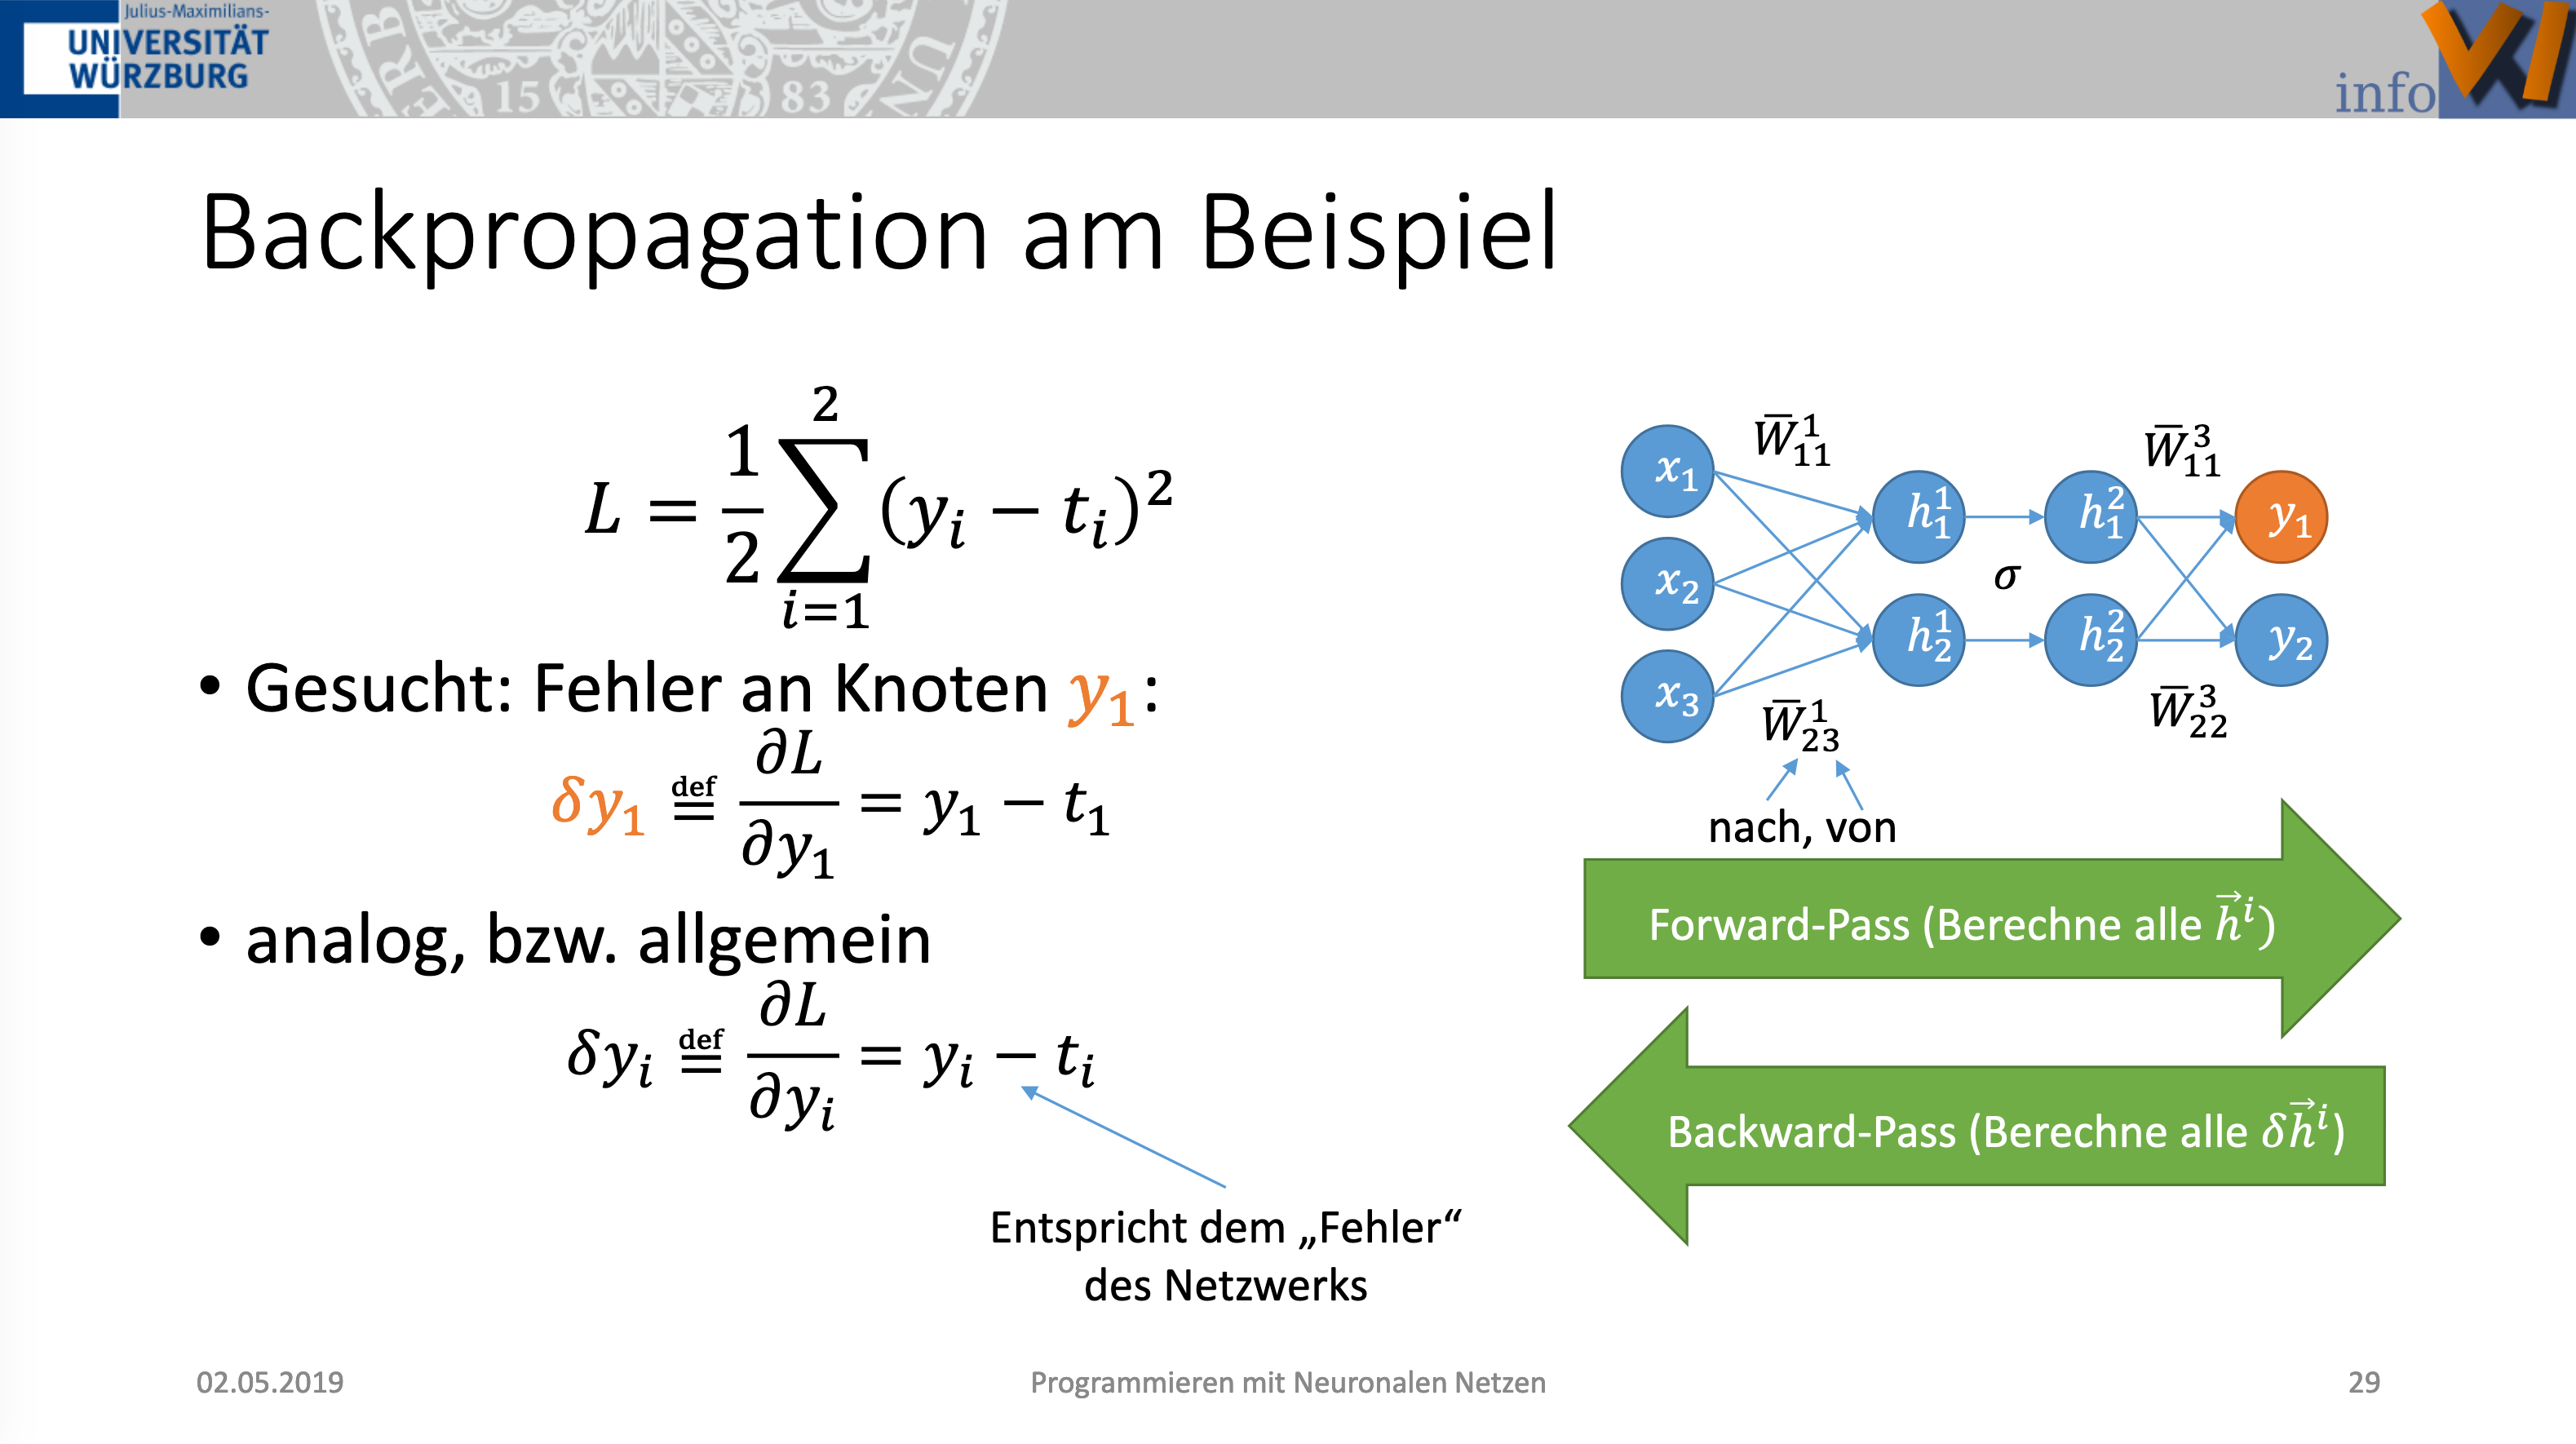
\includegraphics[width=\linewidth]{figures/backpropagation.png}\\
	\textbf{Berechnung der Gewicht-Deltas} Bilden der partiellen Ableitung für jedes Gewicht jedes Layers und Speichern der Werte als Deltas. Zur Berechnung sind die Deltas der Outputs (siehe Backward-Pass) erforderlich. Für Batches werden die Deltas der Gewichte aufsummiert und nach dem Batch geupdated.\\
	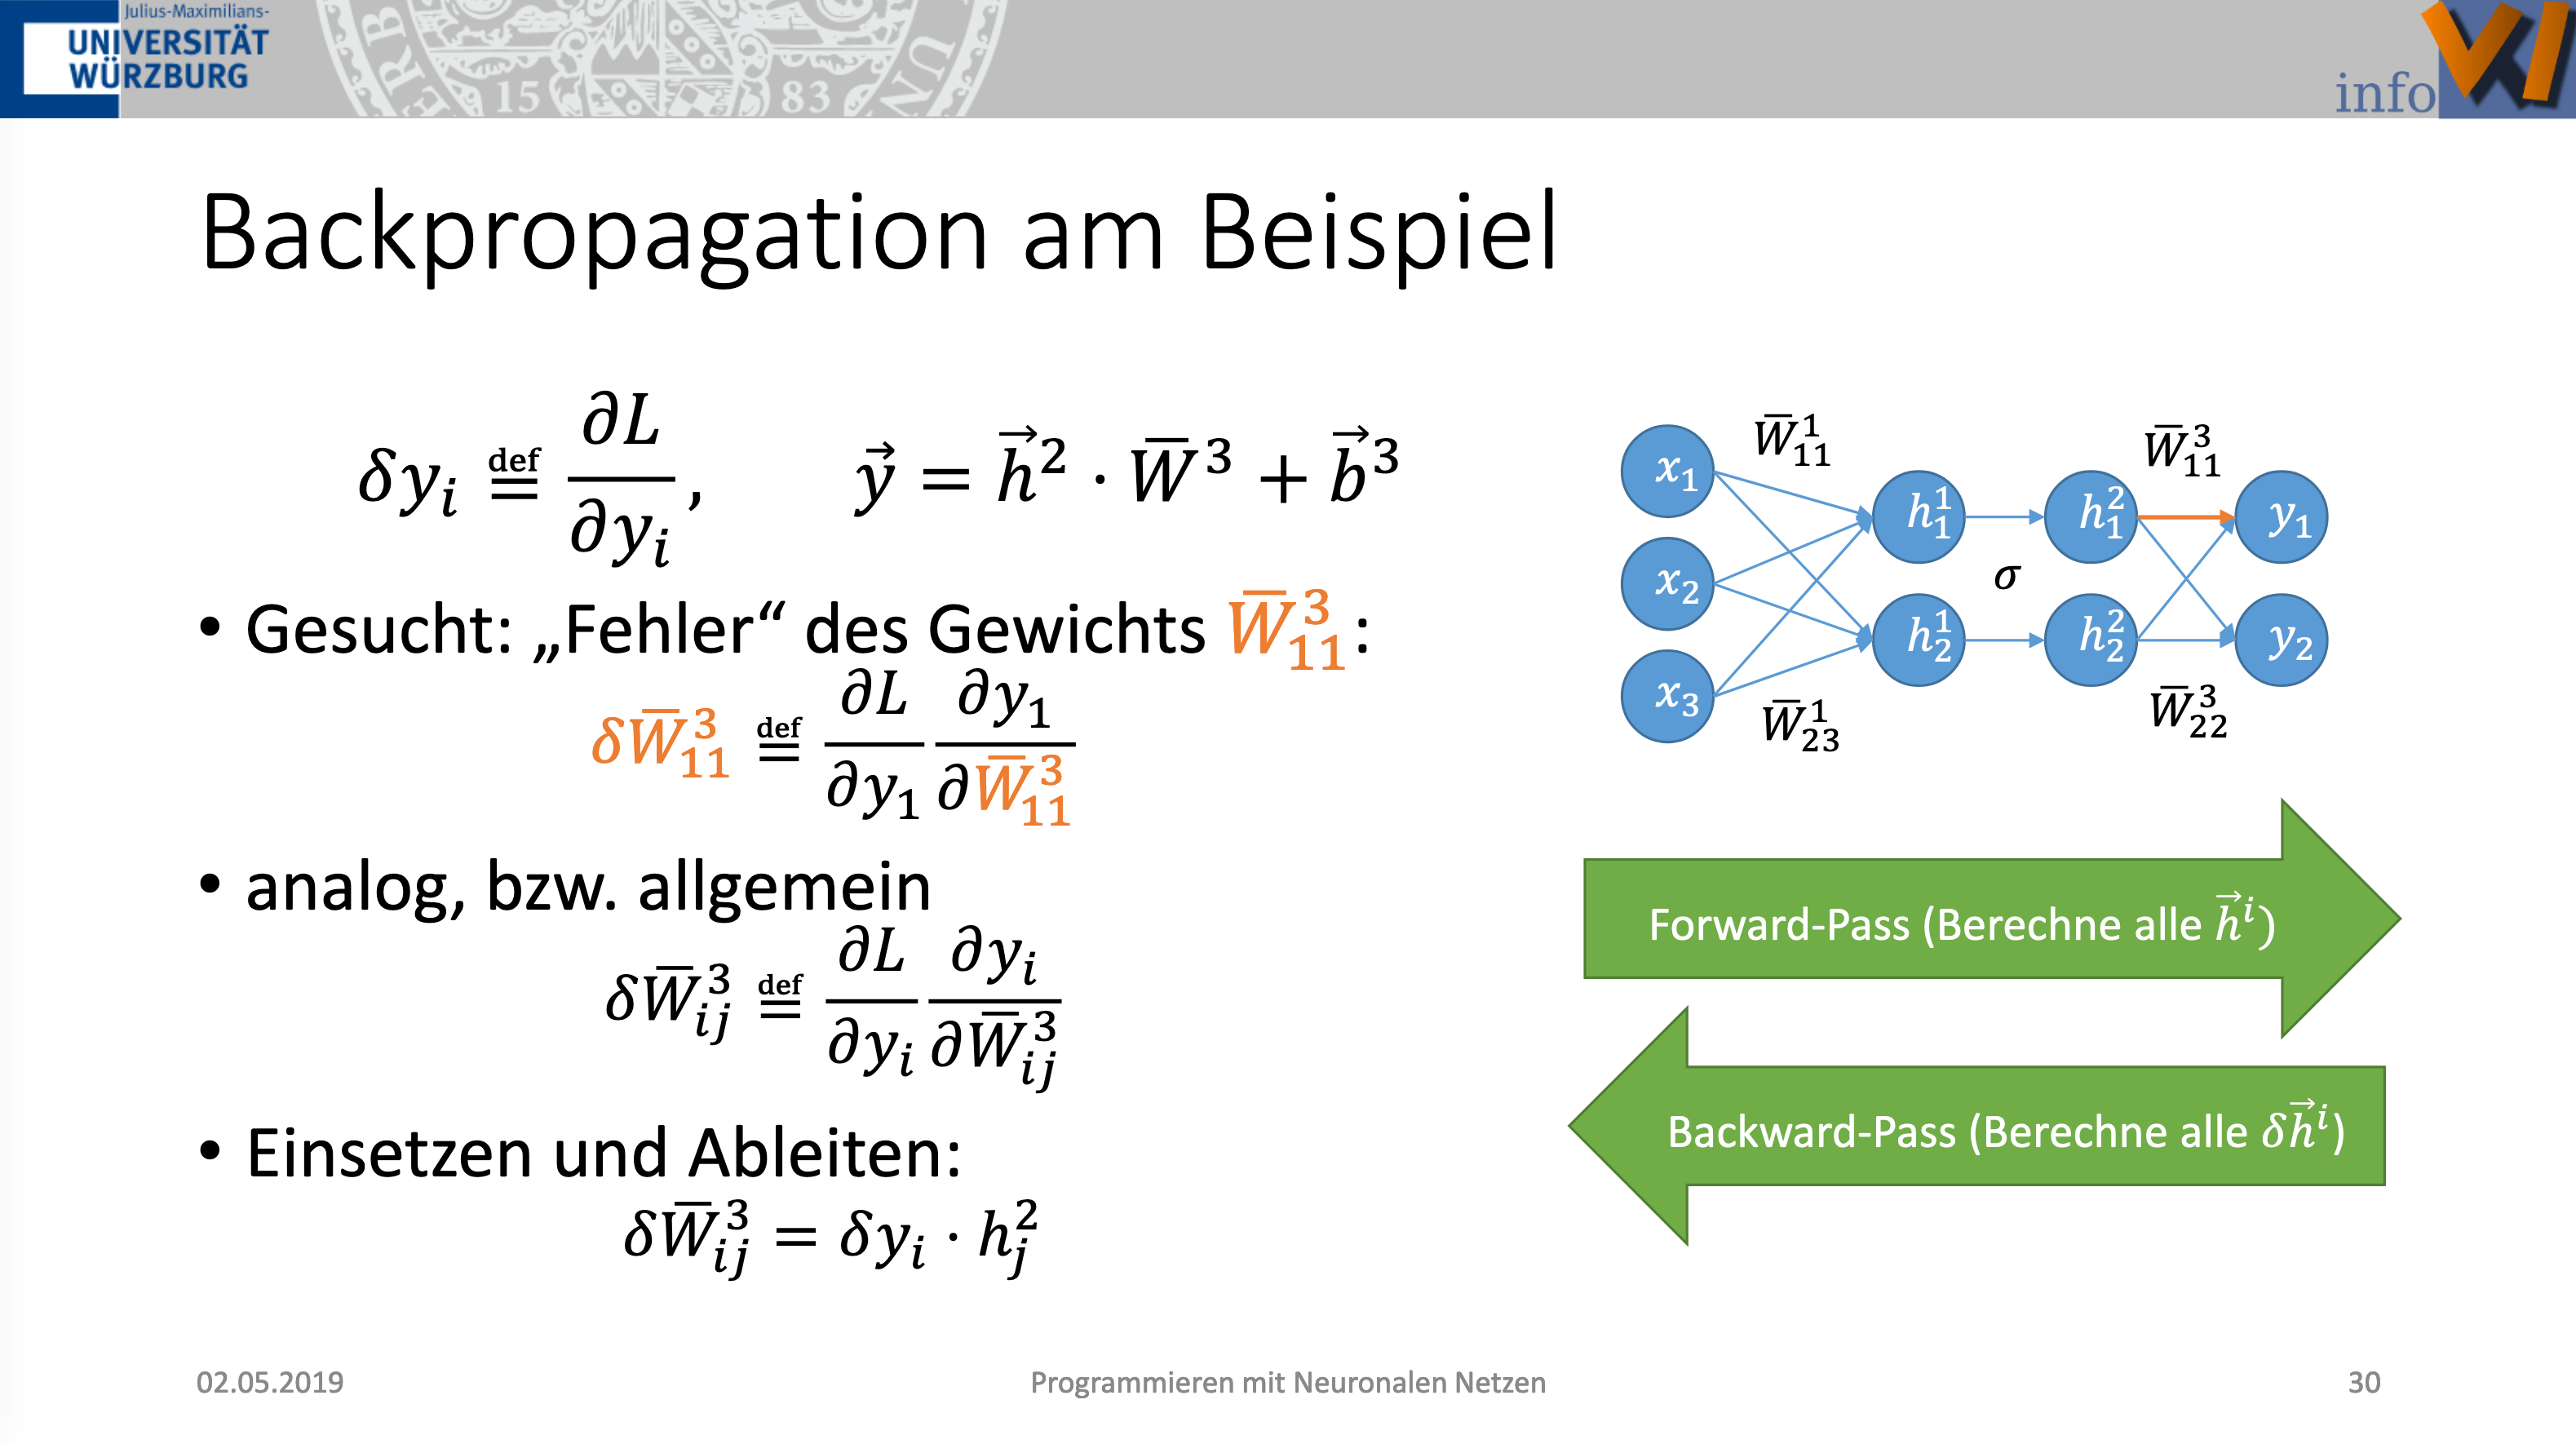
\includegraphics[width=\linewidth]{figures/calculate-delta-weights.png}\\
	\textbf{Update der Gewichte} Die Gewichte werden nun geupdated, in dem die Deltas der Gewichte mit den ursprünglichen Gewichten verrechnet werden. Dafür wird ein Optimierungsverfahren verwendet (siehe unten).\\
	\textbf{Pre-Training} Verwende Startgewichte, die bereits auf ähnlichen Daten trainiert wurden $\rightarrow$ besser als zufällige Initialisierung.\\
	\textbf{Transferlearning} Verwende vortrainiertes Netz und trainiere nur einzelne Schichten (z.B. letzte Schicht für Klassifikation) neu.

	\subsection{Optimizer}
	Optimierungsverfahren sind für das Update der Gewichte zuständig. Sie werden über die Learningrate $\eta$ eingestellt.\\
	\textbf{Gradient Descent} für Gewicht:
	$$w'_{ij} = w_{ij} - \eta \cdot \delta w_{ij}$$
	\textbf{Momentum} simuliert Ball, der die Funktion nach unten rollt:
	$$w_{ij}' = w_{ij} + (mu \cdot v - \eta \cdot \delta w_{ij})$$
	mit $v$ aktuelle Ballgeschwindigkeit, $mu$ wie viel $v$ der Ball behalten soll\\
	\textbf{Nesterov Momentum} verhindert hinauslaufen über Ziel (Minimum) (Problem bei Momentum) $\rightarrow$ verwende Lookahead für Gradient an nächster Position
	$$w_{ij}' = w_{ij} + (mu \cdot v - \eta \cdot \frac{df}{dx}(w_{ij} + mu \cdot v))$$
	\textbf{Adagrad} Verwendet Cache pro Parameter, um variable, sich optimierende Learningrate zu nutzen $\rightarrow$ kleinere Learningrate für große Gewichtsupdates und umgekehrt
	$$cache_{ij} += \delta w_{ij}^2$$
	$$w_{ij}' = w_{ij} -\frac{\eta}{\sqrt{cache_{ij}} + \epsilon} \cdot \delta w_{ij}$$
	\textbf{RMSProp} Sanftere Learningrate/Cache-Anpassung als Adagrad. Update wie bei Adagrad.
	$$cache_{ij}' = decayrate \cdot cache_{ij} + (1 - decayrate) \cdot \delta w_{ij}^2$$
	\textbf{Adam-Optimizer} RMSProp mit Momentum, funktioniert oft am bestehen
	$$m' = \beta_1 \cdot m + (1 - \beta_1) \cdot \delta w_{ij}$$
	$$v' = \beta_2 \cdot v + (1 - \beta_2) \cdot \delta w_{ij}^2$$
	$$w_{ij}' = w_{ij} -\frac{\eta}{\sqrt{v'} + \epsilon} \cdot m'$$

	\subsection{Regularisierung}
	Methoden um Overfitting vorzubeugen
	\begin{itemize}
		\item Rauschen auf Eingabedaten, Gewichten, Ausgabe (Zufallswerte hinzufügen)
		\item Datenaugmentierung
		\item Early-Stopping: Laufende Validierung auf Validierungsset, Trainingsabbruch wenn Accuracy abnimmt
		\item Dropout (siehe Layer)
	\end{itemize}
	\textbf{L2 Regularisierung} Zusatzterm in Lossfunktion: $L_{reg} = L + \frac{1}{2} \lambda \sum_w w^2$\\
	\textbf{Weight Decay} Zusatzterm zur Ableitung der Lossfunktion

	\subsection{Initializer}
	Es gibt mehrere Ansätze die Gewichte vor dem Training initial zu belegen.\\
	\textbf{Random} zufällige Belegung $\rightarrow$ Normalisierung mit Anzahl der Gewichte $n$: $x = \frac{random}{\sqrt{n}}$\\
	\textbf{Glorot/Xavier} Funktioniert am besten für Sigmoid oder Tanh Aktivierung: $x = \frac{random}{\sqrt{\frac{2}{n_{in} + n_{out}}}}$\\
	\textbf{He/Kaiming} Funktioniert am besten für ReLU Aktivierung: $x = \frac{random}{\sqrt{\frac{2}{n_{in}}}}$\\

	\subsection{Netzarchitektur}
	\textbf{Perceptron} (= künstliches Neuron) stellt lineare Trennung (binäre Klassifikation) dar. Kann Funktionen AND, OR und NOT lernen, nicht aber XOR.\\
	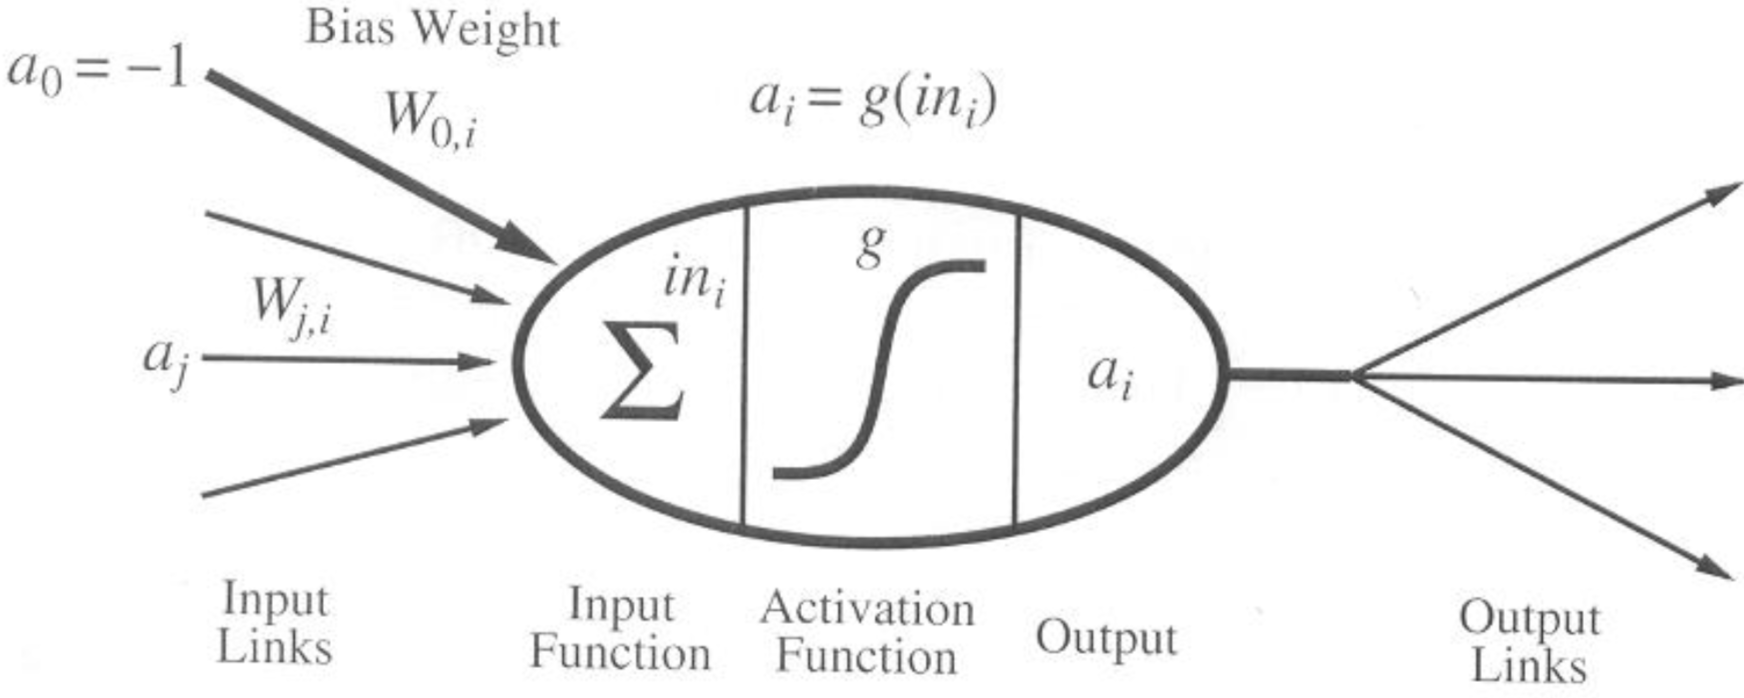
\includegraphics[width=\linewidth]{figures/perceptron.png}\\
	mit Inputs $a_j$ gewichtet mit $W_{ji}$ (ergeben zusammen die Gewichtsmatrix $W$), addiert mit Bias $b$, Outputs $a_i$ und der Aktivierungsfunktion $g$ mit der der Output berechnet wird.
	$$Ausgabe_{Schicht(x)} = g(Eingabe_{Schicht(x)} \cdot W + b) = Eingabe_{Schicht(x+1)}$$
	\textbf{Aktivierungsfunktion} muss bei Multi-Layer-Perceptronen (MLP) nicht-linear sein, da sonst nicht mehr Information gespeichert werden kann.
	$$(x \cdot W + b) \cdot V + a = x \cdot W \cdot V + b \cdot V + a = x \cdot W' + b'$$
	\textbf{Circuit Diagram} Darstellung eines neuronalen Netz als Graph mit Basis-Rechenoperationen. Kann für Forward- und Backwardpass verwendet werden.\\
	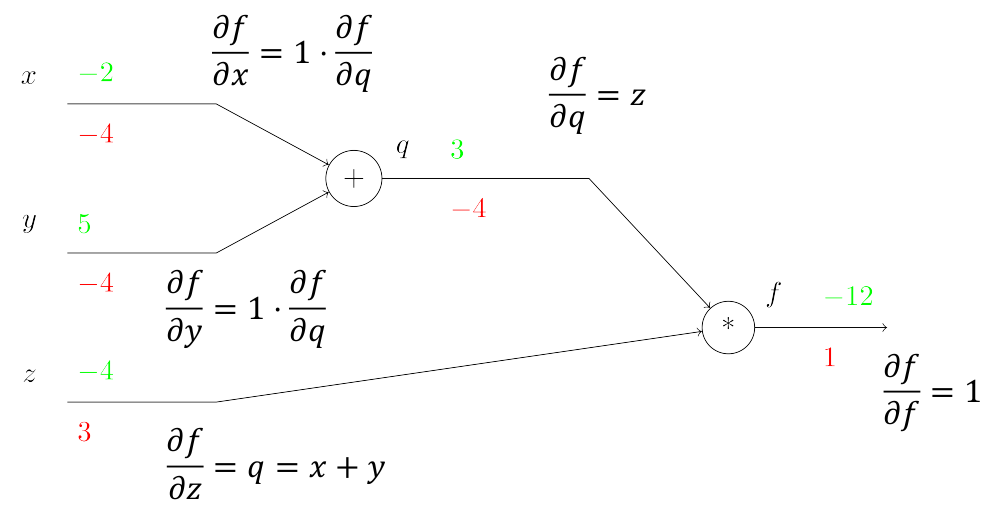
\includegraphics[width=\linewidth]{figures/circuit-diagram.png}\\
	\textbf{Prediction Temperature} Skaliert die Wahrscheinlichkeiten des Softmax. Wenn über Wahrscheinlichkeiten gesampled wird (z.B. bei Textgenerierung) können damit eher sichere oder eher unsichere Vorhersagen gemacht werden.
	$$pred' = pred^{\frac{1}{temp}}$$
	mit $temp \in [0,1]$

	\section{Layer}
	Mögliche Schichten aus denen ein neuronales Netz bestehen kann.
	\subsection{Fully Connected / Dense}
	Voll verbundene Schicht, d.h. jeder Input landet in jedem Neuron. Wird z.B. als letzter Layer zur Klassifikation verwendet, um Vektor mit Logits für Klassen auszugeben.\\
	\textbf{Parameter} $X \in \R^{1 \times a}$: Eingabe, $W \in \R^{a \times n}$: Gewichtsmatrix, $b \in \R^{1 \times n}$: Bias, $n$: Anzahl der Neuronen, $Y \in \R^{1 \times n}$: Ausgabe\\
	\textbf{Forward-Pass} $$Y = X \cdot W + b$$
	\textbf{Backward-Pass} $$\delta X = \delta Y \cdot W^T$$
	\textbf{Calculate Delta Weights} $$\frac{\delta L}{\delta W} = X^T \cdot \delta Y$$ $$\frac{\delta L}{\delta b} = \delta Y$$
	\subsection{Aktivierungsfunktion}
	Elementweise Anwendung\\
	\begin{tabular}{|l|l|l|}
	\hline
	\textbf{Funktion} & \textbf{Forward} & \textbf{Backward}\\
	\hline
	tanh & $Y = \tanh(X)$ & $\delta X = (1 - \tanh^2(X)) \odot \delta Y$\\
	\hline
	Sigmoid & $Y = \sigma(X) = \frac{1}{1 + e^{-X}}$ & $\delta X = (\sigma(X) \cdot (1-\sigma(x))) \odot \delta Y$\\
	\hline
	ReLU & $Y = ReLU(X)$ & $\delta X = ReLU'(X) \odot Y$\\
	\hline
	\end{tabular}\\
	\\
	ReLU: $ReLU(x) = x > 0 ? x : 0$, $ReLU'(x) = x > 0 ? 1 : 0$
	\subsection{Softmax}
	Normalisiert eine Menge von Werten, sodass deren Summe 1 ergibt. Wird zur Berechnung der Wahrscheinlichkeitsverteilung bei Klassifikation verwendet.\\
	\textbf{Forward-Pass} $$Y = softmax(X) = \frac{e^{x_i}}{\sum_i e^{x_i}}$$
	\textbf{Backward-Pass} $$\delta X = \delta Y \cdot
	\begin{bmatrix}
	\frac{\delta y_1}{\delta x_1} & \cdots & \frac{\delta y_n}{\delta x_1}\\
	\cdots & \ddots & \cdots\\
	\frac{\delta y_1}{\delta x_n} & \cdots & \frac{\delta y_n}{\delta x_n}
	\end{bmatrix}
	$$
	\subsection{Dropout}
	Für Regularisierung verwendet. Ein Teil der Gewichte wird zufällig je Durchlauf auf 0 gesetzt (deaktiviert). Wird nicht trainiert, sollten alle Gewichte weitergegeben, aber durch die Dropout-Rate geteilt werden, da sonst eine zu hohe Aktivierung der nächsten Schicht statt findet.\\
	\textbf{Parameter} $d$: Dropout-Rate gibt den prozentualen Anteil der zu deaktivierenden Gewichte an.
	\subsection{Convolutional}
	Extrahiert Features aus einer Matrix. Wird oft in der Bildklassifizierung verwendet oder NLP zur Satzklassifikation (Kernel Größe der Embeddings $\times$ Anzahl betrachteter Wörter).\\
	\textbf{Beispiel für NLP}\\
	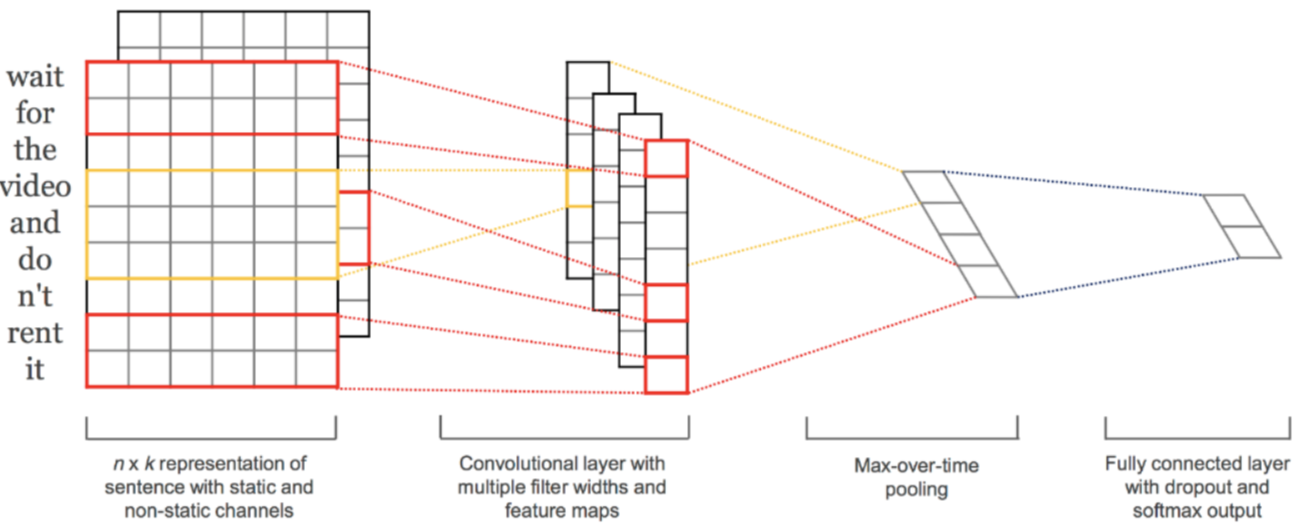
\includegraphics[width=\linewidth]{figures/convolution-nlp.png}\\
	\textbf{Parameter}\\
	$X \in \R^{h \times w \times d}$: Eingabe\\
	$(fh, fw)$: Filtergröße\\
	$fn$: Anzahl Filter\\
	$F \in \R^{fh \times fw \times fd \times fn}$: Filtertensor\\
	$b \in \R^{fn}$: Bias (ein Wert pro Ausgabechannel, wird auf jeden Wert des Channels addiert)\\
	$Y \in \R^{(h-fh+1) \times (w-fw+1) \times fn}$: Ausgabe\\
	\textbf{Optionale Parameter} Stride: wie weit der Filter verschoben wird (default = 1), Dilation: zusätzliche 0en im Filter (Filter über nicht benachbarte Elemente)\\
	\textbf{Padding} Covolution verkleinert die Daten. Um dies zu verhindern, kann die Eingabe gepadded werden (Hinzufügen von 0en am Rand der Eingabe).\\
	\textit{Half-Padding}: Ausgabegröße = Eingabegröße, $ph = \lfloor \frac{fh}{2} \rfloor$, $pw = \lfloor \frac{fw}{2} \rfloor$\\
	\textit{Full-Padding (Full-Convolution)}: Ausgabegröße $>$ Eingabegröße, $ph = fh - 1$, $pw = fw - 1$\\
	\textbf{Forward-Pass} $*$ bezeichnet die Faltungsoperation\\
	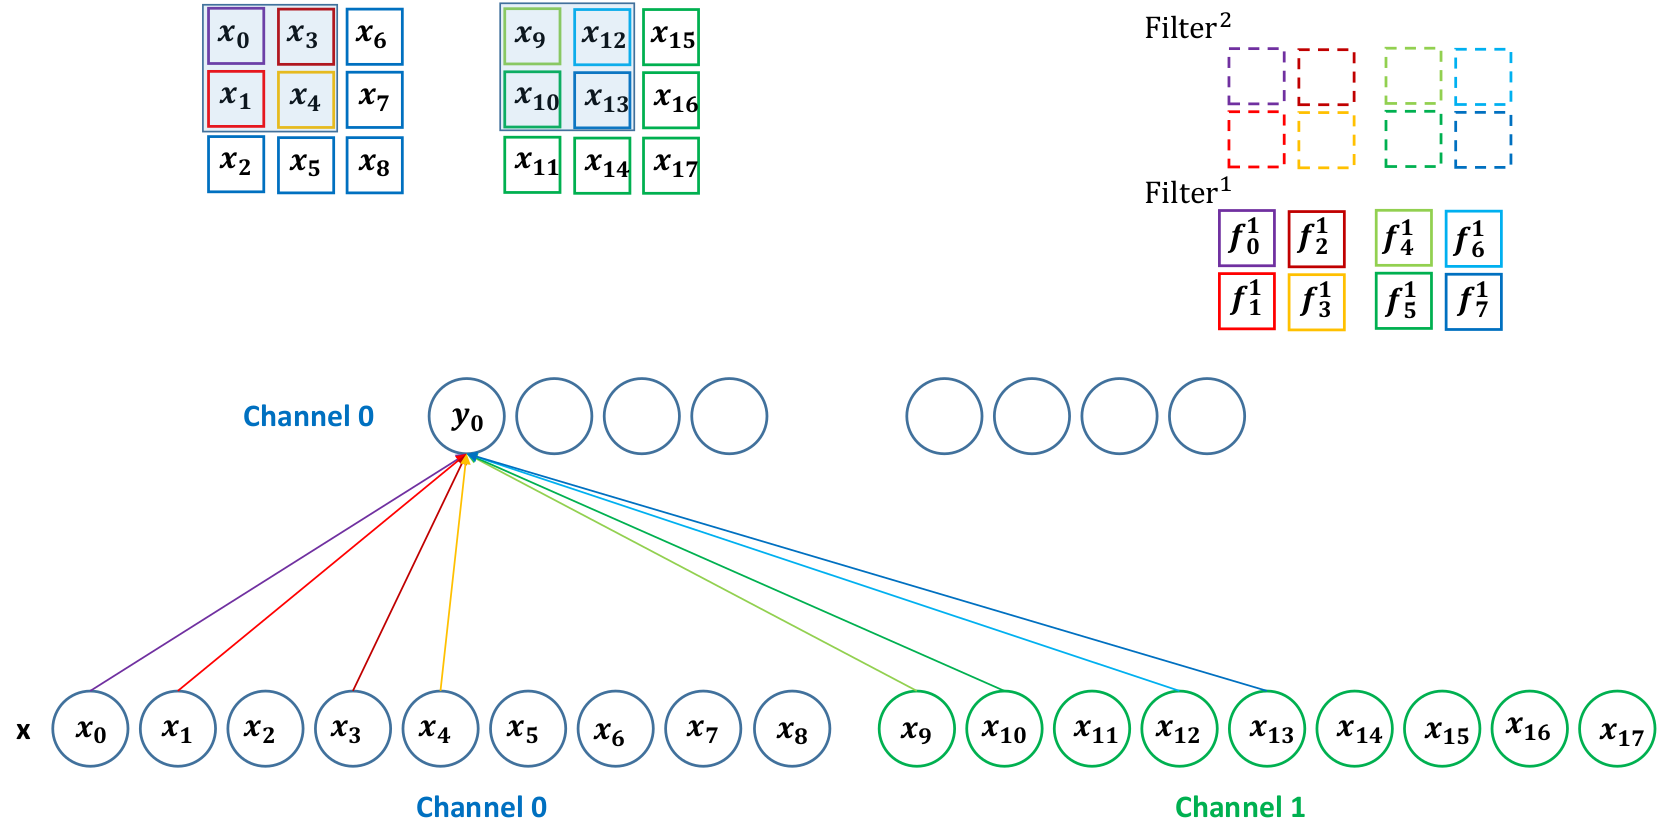
\includegraphics[width=\linewidth]{figures/convolution.png}
	$$Y = X * F + b$$
	\textbf{Backward-Pass} $*_F$ bezeichnet die Full-Convolution\\
	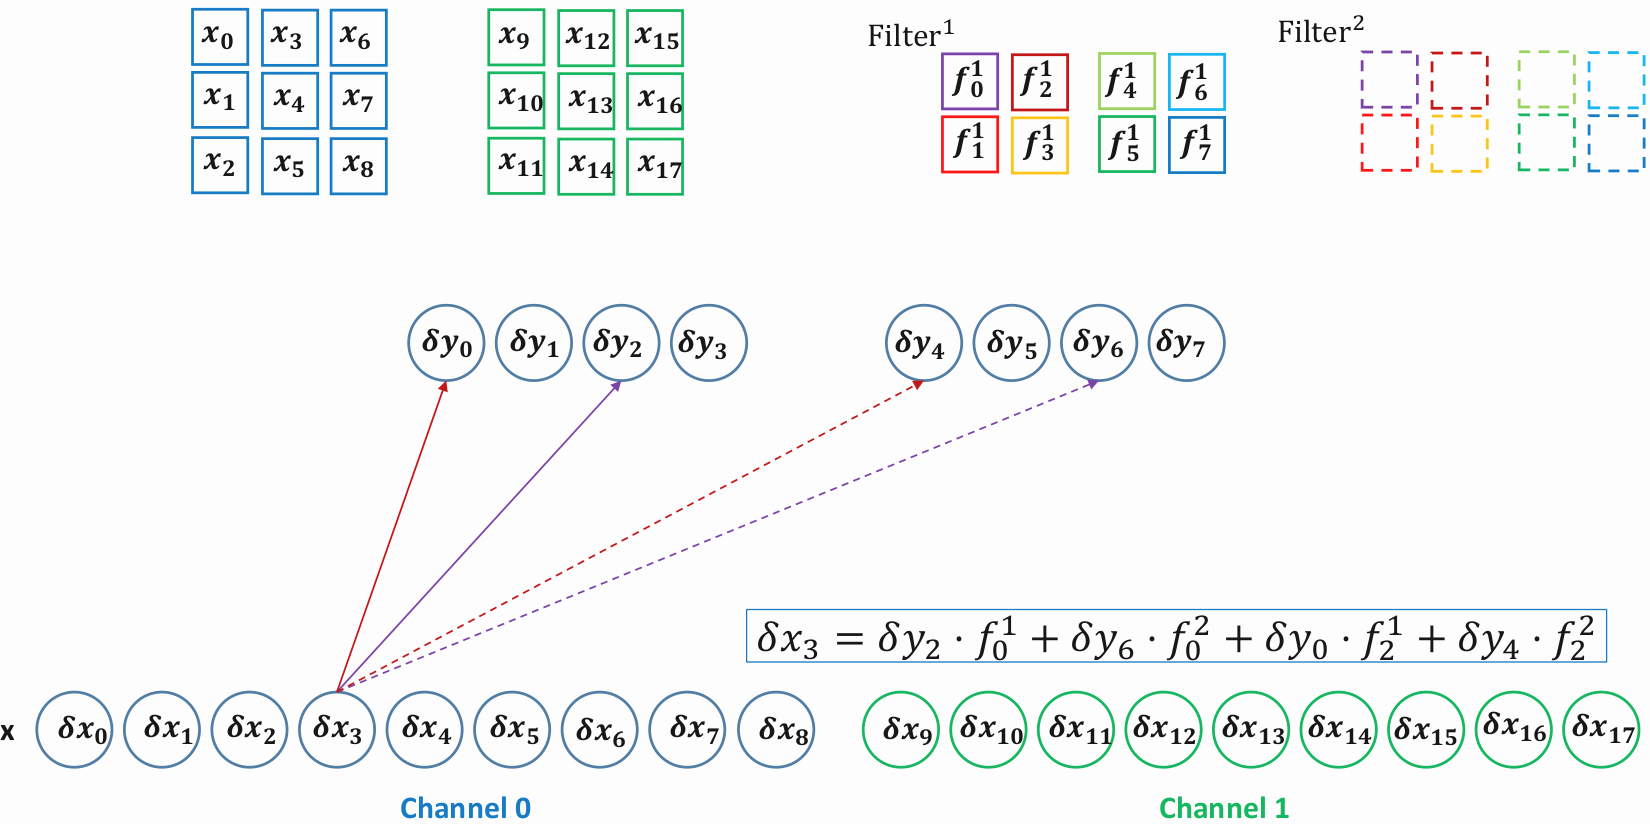
\includegraphics[width=\linewidth]{figures/convolution-backward.png}
	$$\delta X = \delta Y *_F rot^{180}_{h,w}(trans(F))$$
	\textbf{Calculate Delta Weights} $*_{ch}$ bezeichnet die Channel-Wise-Convolution, $f$ ist ein Element des Filtertensors
	$$\frac{\delta L}{\delta f} = X *_{ch} \delta Y$$
	$$\frac{\delta L}{\delta b_f} = \sum_i \delta y_{i,f}$$
	\subsection{Pooling}
	Reduziert die Werte innerhalb eines Filters auf einen Wert (z.B. Maximum oder Durchschnitt). Filter wird ohne Überlappung (mit Stride) verschoben.\\
	\textbf{Forward-Pass}\\
	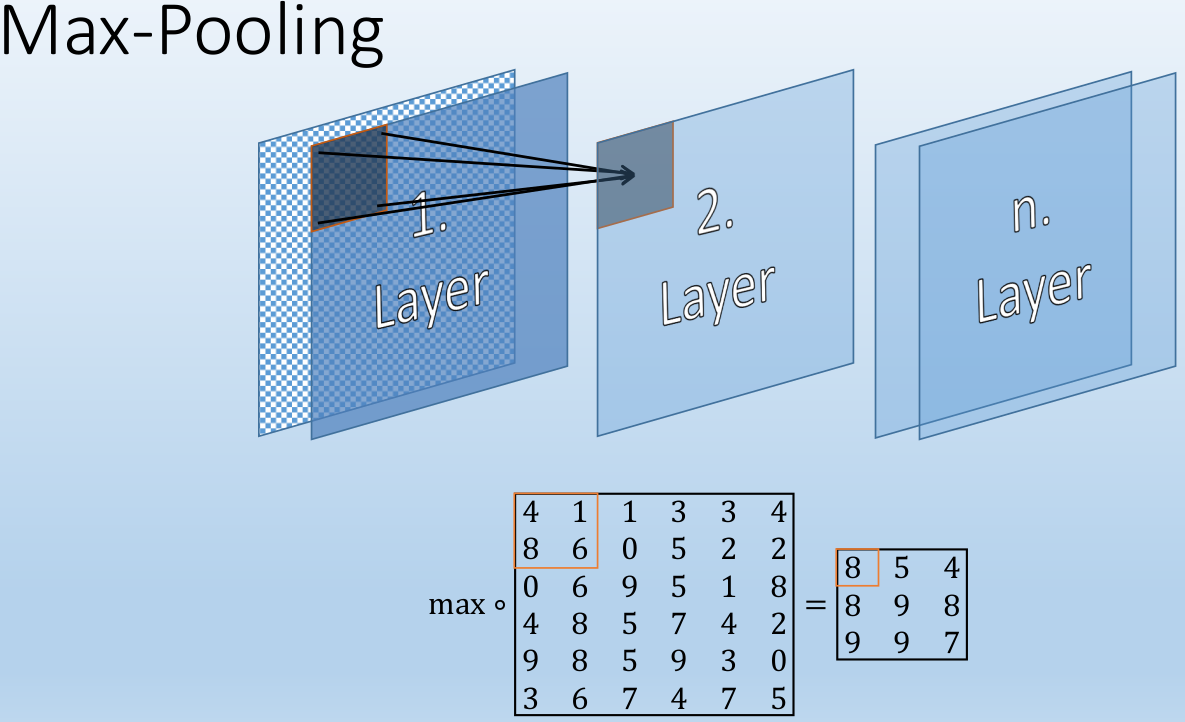
\includegraphics[width=\linewidth]{figures/max-pooling.png}\\
	\textbf{Backward-Pass} Nur die Elemente, die im Forward-Pass an der Berechnung des Outputs beteiligt waren, bekommen anteilig oder ganz das Delta des jeweiligen Outputs.
	$$\delta x_i = (x_i == max) ? \delta y : 0$$
	\textbf{Maximum over time pooling} Übernimmt den größten Wert pro Outputvektor eines Filters
	\subsection{Vanilla RNN}
	Recurrent Neuronal Networks (RNNs) werden verwendet, um Daten unterschiedlicher Länge zu verarbeiten. Dabei wird ein Hidden State $h$ in jedem Schritt um Informationen der Eingabe ergänzt.\\
	\textbf{Parameter}\\
	$[x_0, \cdots, x_n] = X \in \R^{n \times m}$: Eingabevektoren mit jeweils Länge $m$\\
	$g$: Zwischenvariable nach der Addition vor $\tanh$\\
	$h$: Hidden State ($h_{-1}$ kann mit Nullen initialisiert werden)\\
	$W_x, W_h, W_o$: Gewichtsmatrizen\\
	$b$: Bias\\
	$[o_0, \cdots, o_n] = O \in \R^{n \times l}$: Ausgabevektoren mit jeweils Länge $l$\\
	\textbf{Funktionsweise}\\
	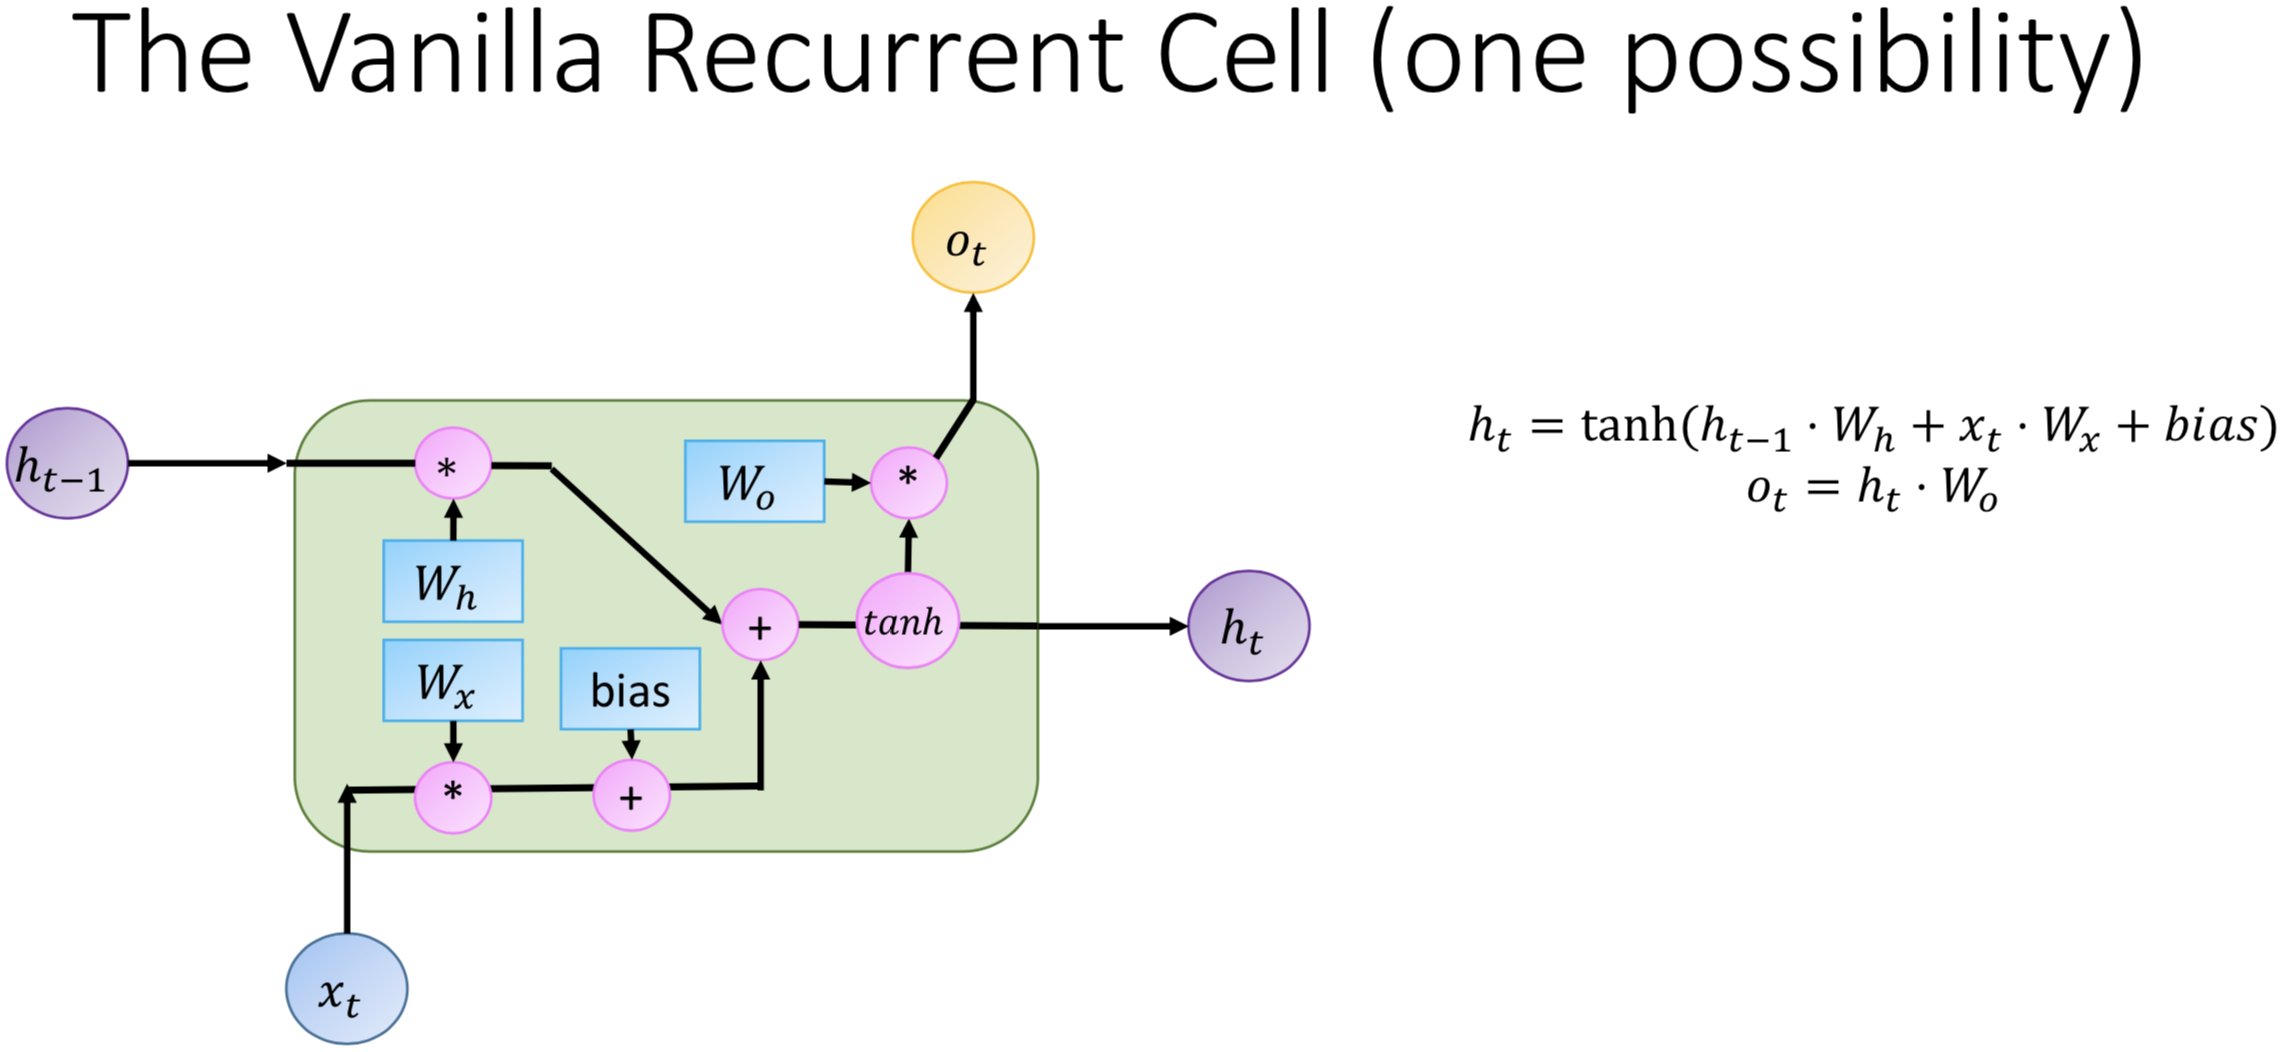
\includegraphics[width=\linewidth]{figures/vanilla-rnn.png}\\
	\textbf{Forward-Pass}
	$$h_t = \tanh(h_{t-1} \cdot W_h + x_t \cdot W_x + b)$$
	$$o_t = h_t \cdot W_o$$
	\textbf{Backward-Pass}
	$$\delta h_t = \delta o_t \cdot W_o^T + \delta g_{t+1} \cdot W_h^T$$
	$$\delta g_t = \delta h_t \cdot (1 - \tanh^2(g_t)) = \delta h_t \cdot (1 - h_t^2)$$
	$$\delta x_t = \delta g_t \cdot W_x^T$$
	\textbf{Calculate Delta Weights}
	$$\delta W_h = \sum_t h_{t-1}^T \cdot \delta g_t$$
	$$\delta W_x = \sum_t x_t^T \cdot \delta g_t$$
	$$\delta W_o = \sum_t h_t^T \cdot \delta o_t$$
	$$\delta b = \sum_t \delta g_t$$
	\subsection{Gru}
	Verwendet zwei Gates (wie $g$ im Vanilla RNN), um zu bestimmen, was aus dem alten Internal State $h$ übernommen wird und was von den aktuell verarbeiteten Daten hinzugefügt wird.\\
	\textbf{Funktionsweise}\\
	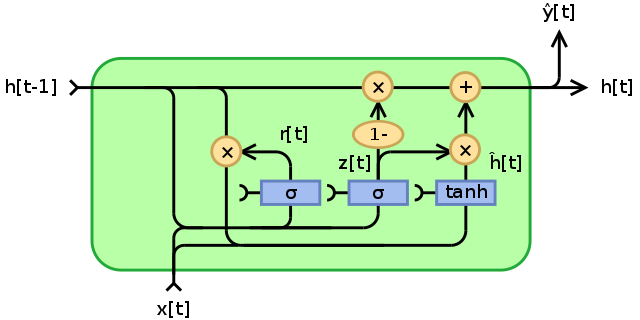
\includegraphics[width=\linewidth]{figures/gru.png}
	\subsection{LSTM}
	Verwendet drei Gates (Forget, Input, Output) und zusätzlichen State $c$\\
	\textbf{Funktionsweise}\\
	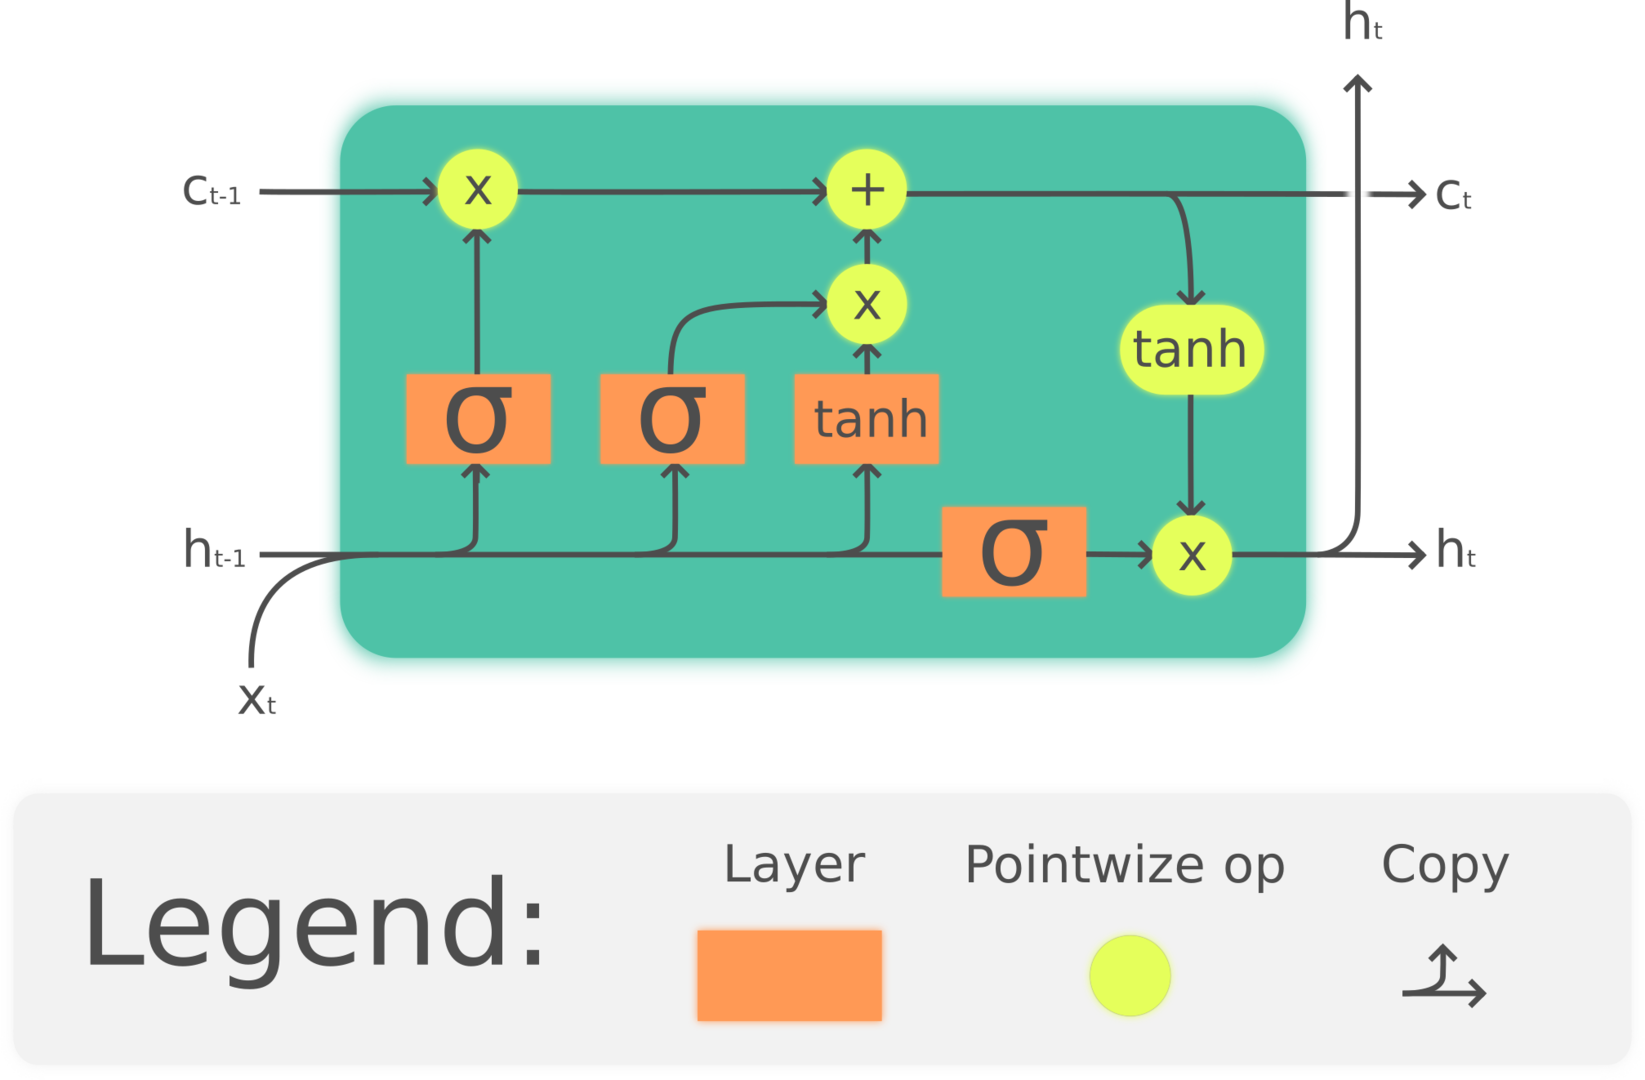
\includegraphics[width=\linewidth]{figures/lstm.png}
	\subsection{Highway Layer}
	Verwendet ein Gate, das bestimmt, ob der Layer wie ein Fully Connected Layer funktioniert oder lediglich den Input weitergibt. Wird verwendet bei sehr tiefen Netzwerken ($>$ 100 Layer), um Daten über lange Zeit/viele Layer hinweg nutzbar zu machen.\\
	\textbf{Forward-Pass}
	$$Y = (X \cdot W + b) \cdot T(x) + x \cdot (1 - T(x))$$
	$$T(x) = \sigma(x \cdot W_T + b_T)$$

	\section{Loss-Funktionen}
	$X$: Eingabe der Loss-Funktion bzw. Ausgabe des Netzes (Prediction)\\
	$T$: Erwartetes Ergebnis (Ground Truth)
	\subsection{Cross Entropy}
	Negative-Log-Likelihood, Cross-Entropy\\
	\textbf{Forward-Pass} $$L = -\sum_i t_i \cdot \log(x_i)$$
	\textbf{Backward-Pass} $$\frac{\delta L}{\delta x_i} = -\frac{t_i}{x_i}$$
	\subsection{Mean Squared Error}
	Euklidischer Loss, Mean-Squared-Error, $l_2$-Loss\\
	\textbf{Forward-Pass} $$L = \sum_i \frac{1}{2} (x_i - t_i)^2$$
	\textbf{Backward-Pass} $$\frac{\delta L}{\delta x_i} = x_i - t_i$$

	\section{Textrepräsentation}
	Wie kann Text (Wörter, Buchstaben) für NLP-Tasks mit neuronalen Netzen repräsentiert werden?\\
	\textbf{Dokument} beschreibt eine Menge an Text, z.B. Satz, Tweet, Buch, etc.\\
	\textbf{Vokabular} alle möglichen Wörter in einem bestimmten Kontext (z.B. Duden für deutsche Sprache)\\
	\textbf{Bag of Words} simpler Ansatz, Vektor der für jedes Wort des Vokabulars einen Wert beinhaltet, Anzahl der Worthäufigkeit im Dokument, Reihenfolge der Wörter im Dokument wird nicht betrachtet\\
	$\rightarrow$ funktioniert gut, aber verliert viel Information über Kontext\\
	\textbf{One-hot-vector} repräsentiert ein Wort, Vektor hat einen Eintrag für jedes Wort des Vokabulars, Eintrag für zu repräsentierendes Wort ist 1 alle anderen 0\\
	$\rightarrow$ Reihenfolge durch Sequenz von one-hot-vectors abbildbar, aber Ähnlichkeiten von Wörtern werden nicht berücksichtigt\\
	\textbf{Cosine-Similarity} Ähnlichkeit von Wörtern über Cosinus Berechnen
	$$sim_{cos}(x,y) = \frac{\sum_{i=1}^N x_i \cdot y_i}{\sqrt{\sum_{i=1}^N x_i^2} \cdot \sqrt{\sum_{i=1}^N y_i^2}}$$
	\textbf{WordNet} handgelabelter Datensatz mit Ähnlichkeitsbeziehungen von Wörtern $\rightarrow$ nicht genau genug, unvollständig, menschlicher Bias\\
	\textbf{Word Embedding} Vektor, der ein Wort repräsentiert. Bekannte Verfahren Embeddings zu erzeugen:\\
	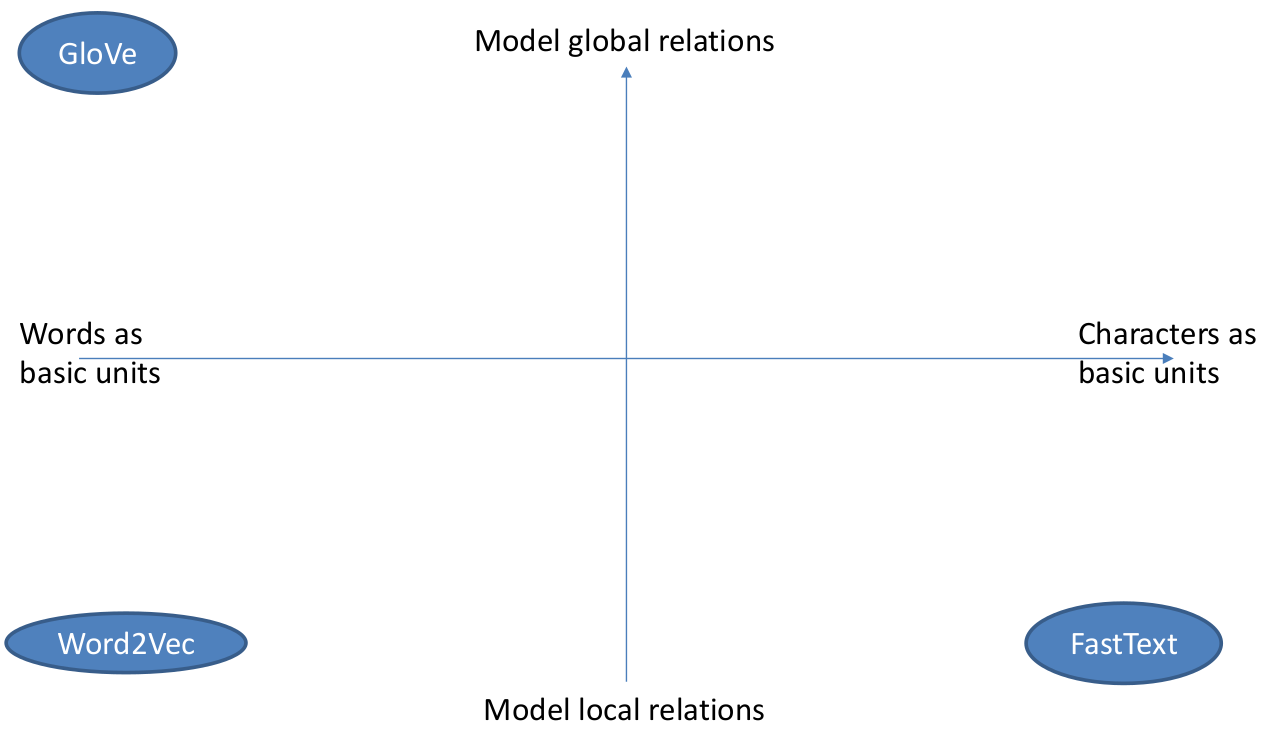
\includegraphics[width=\linewidth]{figures/word-embeddings.png}\\

	\subsection{Word2Vec}
	Annahme: Ähnliche Wörter kommen im ähnlichen Kontext vor d.h. sie sind in Texten häufig von den gleichen Wörtern umgeben.\\
	Berechnung von Word Embeddings (feste Länge) anhand der häufig dieses Wort umgebenden Wörter $\rightarrow$ ähnliche Wörter bekommen ähnliche Vektoren\\
	Word2Vec wird selbst auf Beispieltexten trainiert\\
	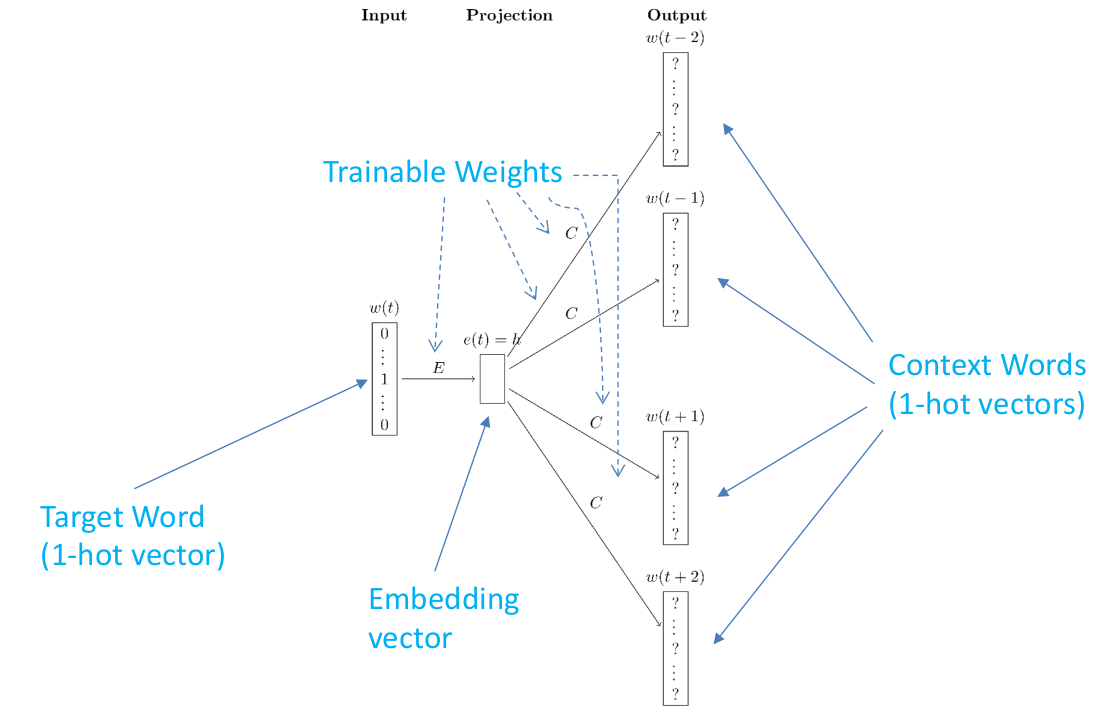
\includegraphics[width=\linewidth]{figures/word2vec-nn.png}\\
	\textbf{CBOW} Center Wort durch Kontextwörter vorhersagen\\
	\textbf{Skip-gram} Kontextwörter durch Center Wort vorhersagen\\
	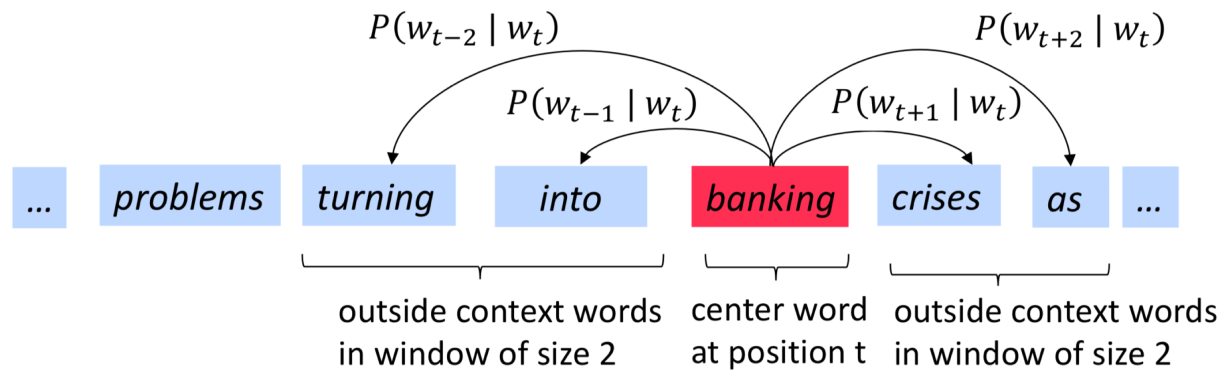
\includegraphics[width=\linewidth]{figures/word2vec.png}

	\subsection{GloVe (Global Vectors)}
	Berechnung von Word Embeddings über eine Matrix $X$, die für einen Wortkorpus die Häufigkeiten angibt, mit der zwei Wörter zusammen auftreten. Verwendet globale Abhängigkeiten statt lokale wie bei Word2Vec.\\
	Neue, unbekannte Wörter werden auf gleichen UNKNOWN-Vektor abgebildet (wie bei Word2Vec).

	\subsection{FastText}
	Funktioniert wie Word2Vec auf lokalem Kontext, aber verwendet Bustaben n-Gramme (Buchstabenketten der Länge $n$) statt ganze Wörter. Word Embeddings werden durch Aufsummieren der Vektoren ihrer n-Gramme erzeugt.\\
	$\rightarrow$ kann neue Wörter besser abbilden, da n-Gramme vermutlich bekannt (z.B. bei konjugierten Verben)\\
	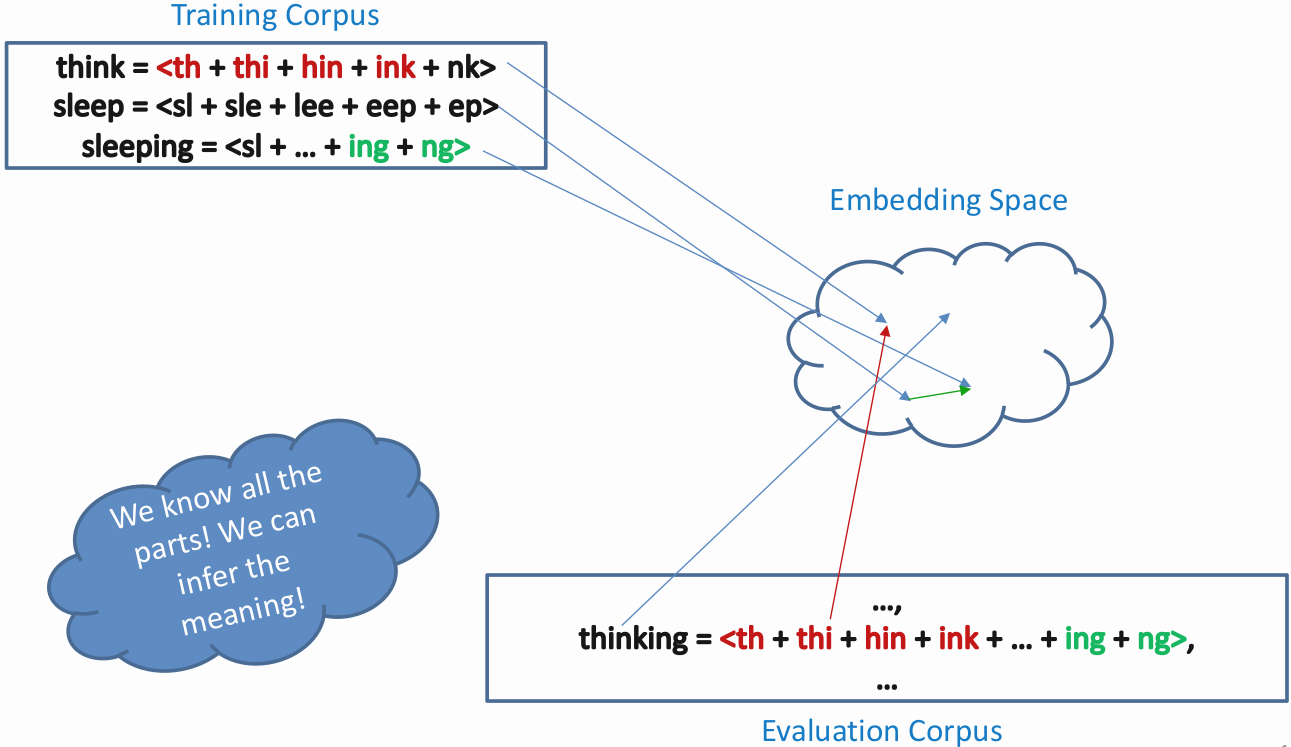
\includegraphics[width=\linewidth]{figures/fasttext.png}

	\subsection{Weltwissen}
	Word Embeddings werden durch die vorgestellen Verfahren nur auf einen bestimmten Korpus angepasst. Menschen verstehen Sprache besser durch Einbeziehen von Hintergrundinformationen, sog. Weltwissen.\\
	\textbf{Quelle für Weltwissen} ist z.B. Dbpedia (maschinenlesbare Form der Wikipedia), Wikidata, BabelNet, ConceptNet (verbindet Begriffe durch gewichtete, beschriftete Beziehungen/Kanten, z.B. Synonym, TeilVon, ...)\\
	\textbf{Pointwise mutual information} Treten zwei Wörter öfters zusammen auf als wenn sie unabhängig wären?
	$$PMI(word_1, word_2) = \log_2 \frac{P(word_1, word_2)}{P(word_1)P(word_2)}$$
	\textbf{ConceptNet Numberbatch} Anreichern von existierenden Embeddings (Word2Vec, GloVe oder FastText) mit Weltwissen aus ConceptNet $\rightarrow$ Abbildung durch neuronales Netz mit Retrofitting Loss-Funktion\\
	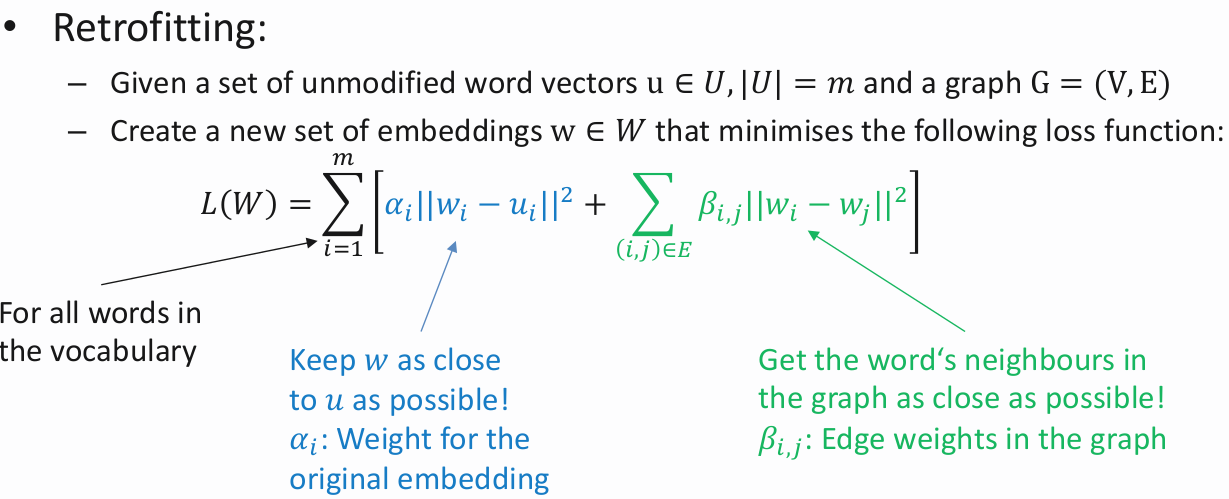
\includegraphics[width=\linewidth]{figures/retrofitting.png}

	\subsection{Evaluation}
	Mehrere Word Embeddings können auf verschiedene Weise miteinander verglichen werden.\\
	\textbf{Extrinsisch} Evaluation durch Verwenden in einem NLP-Task\\
	\textbf{Intrinsisch} hand-annotierten Evaluationsdatensatz (Human Intuition Datasets HID, z.B. WS-353, MEN-3000, ...) mit Wortpaaren verwenden, der Ähnlichkeitsgrad vorhersagt, z.B. r(table, chair) $>$ r(duck, plane)\\
	$\rightarrow$ Word Embeddings können auch auf HIDs nachtrainiert werden

	\section{Anwendungsfelder für NLP}
	\subsection{Textklassifikation}
	Abbilden eines Textes auf ein Label\\
	\textbf{Sentimentanalyse} Ausgabe eines Stimmungswertes für einen Text meist zwischen -1 (negativ) und 1 (positiv).

	\subsection{Textgenerierung}
	Führt vorgegebenen Text weiter. Perfekter Text Generator besteht Turing Test
	
	\subsection{Machine Translation}
	Maschinelle Übersetzung verwendet RNNs wodurch folgende Probleme entstehen:
	\begin{itemize}
		\item unterschiedliche Satzstellung bei verschiedenen Sprachen
		\item ein Inputwort entspricht nicht gleich einem Outputwort (z.B. neben $\Rightarrow$ next to)
	\end{itemize}
	$\rightarrow$ \textbf{Encoder-Decoder-Architektur} liest gesamten Satz mit einem RNN ein und erzeugt mit anderem RNN die Ausgabe\\
	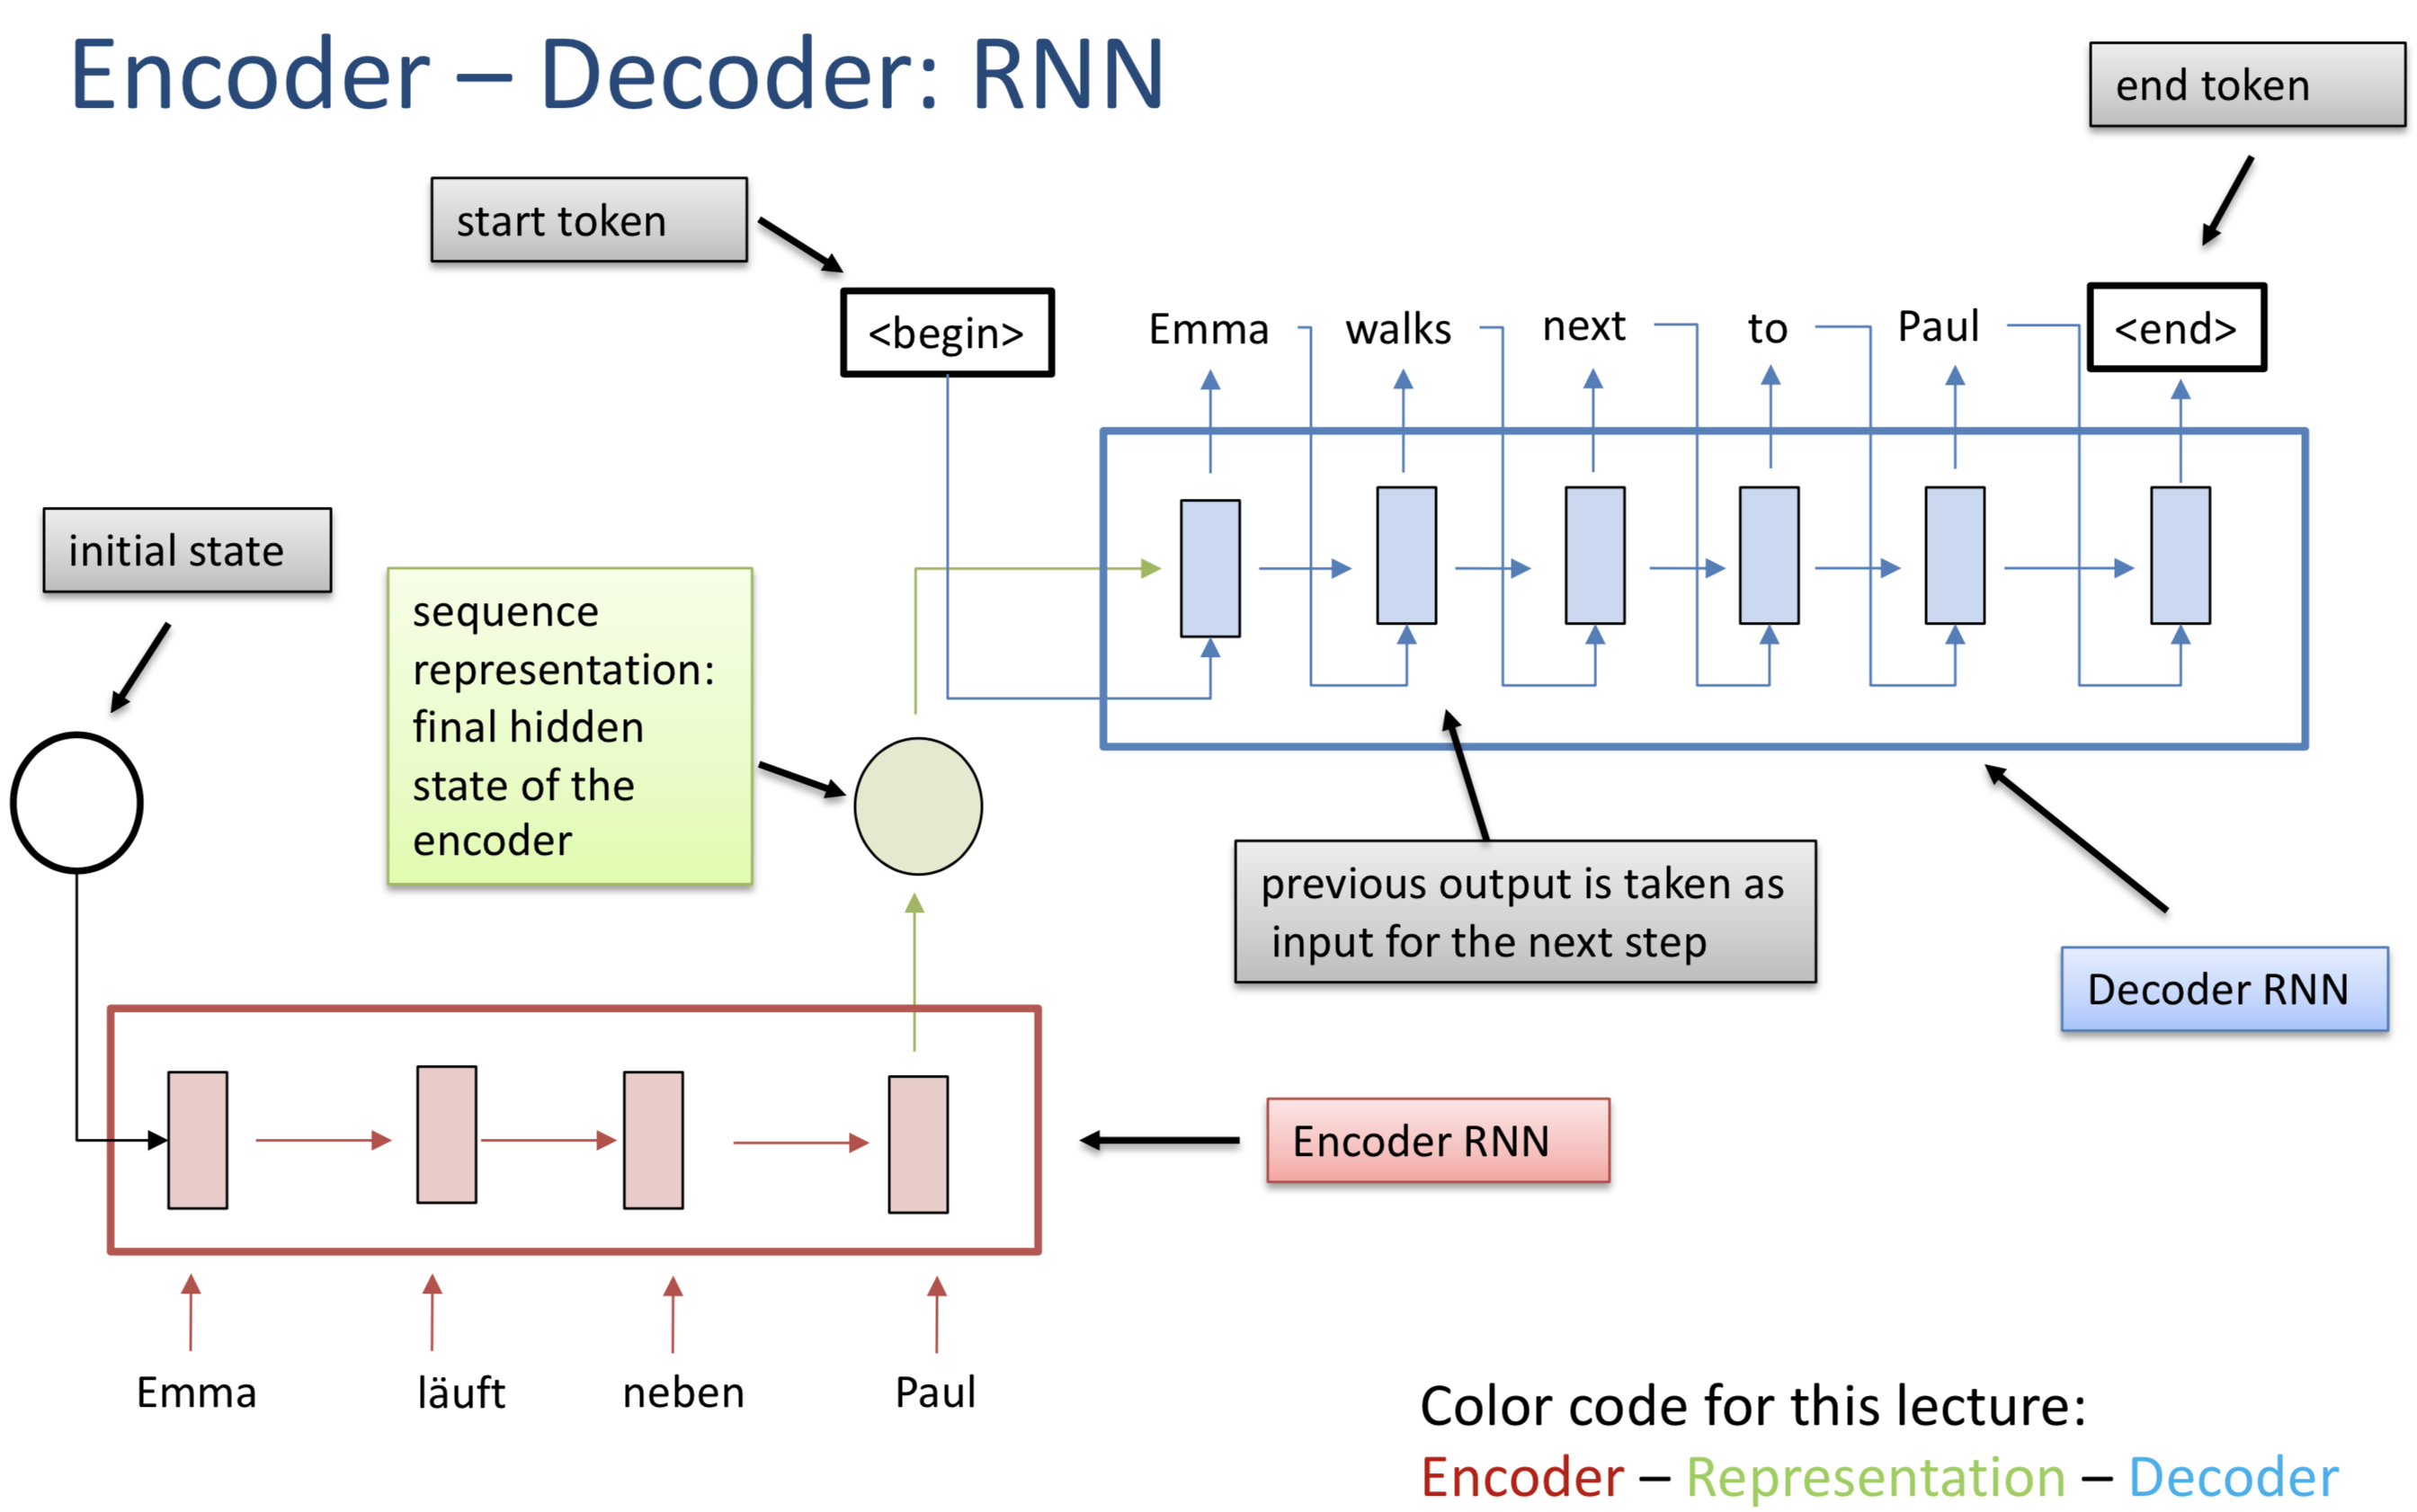
\includegraphics[width=\linewidth]{figures/encoder-decoder-rnn.png}\\
	\textbf{Teacher Forcing} Ausgabewort ist Eingabe für nächsten Decoderschritt. Um Fehler zu vermeiden, solle die Eingabe für den nächsten Schritt das vorherige Wort der Ground Truth sein.\\
	$\rightarrow$ sollte nur zu Beginn des Trainings verwendet werden, dann Wort der vorherigen Vorhersage, da Netzwerk sich sonst darauf verlässt etwas richtiges zu bekommen\\
	\textbf{Greedy Search} immer wahrscheinlichstes Wort nehmen\\
	\textbf{Beam Search} betrachte die $B$ Sequenzen mit der höchsten Wahrscheinlichkeit und entscheide später für die beste ($B = 1 \rightarrow$ Greedy-Search)\\
	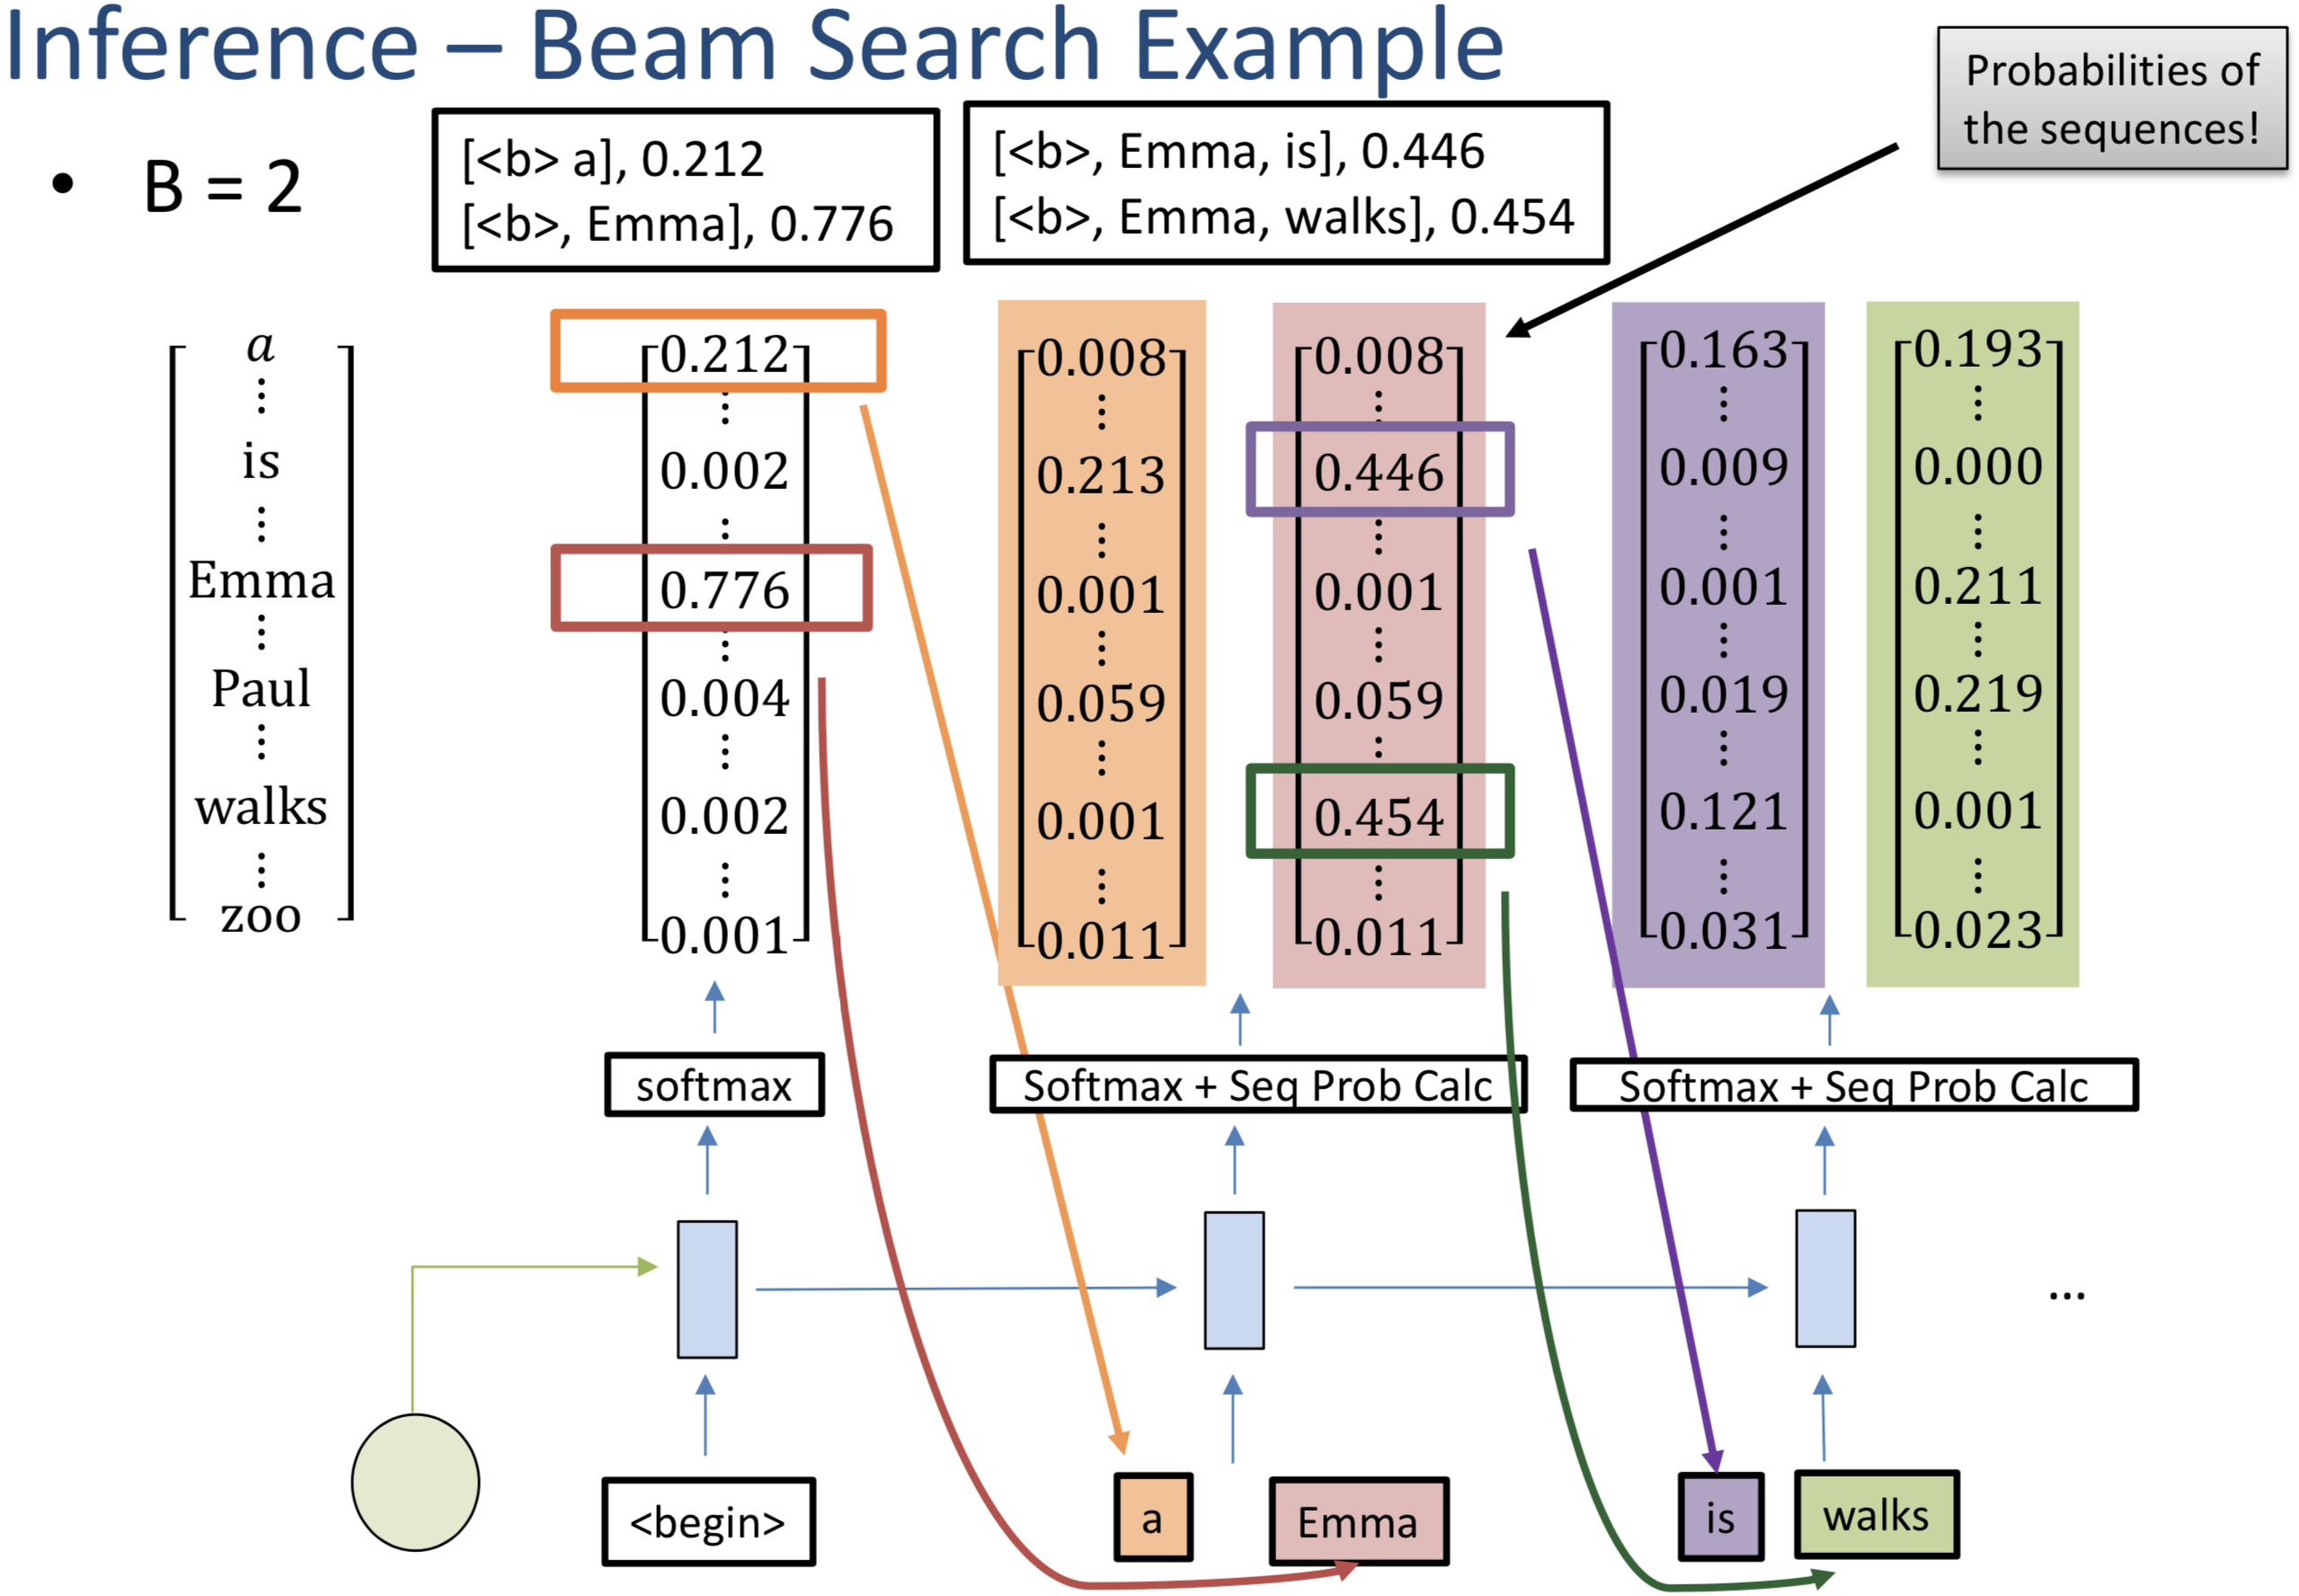
\includegraphics[width=\linewidth]{figures/beam-search.png}\\
	\textbf{BiRNN} zwei RNNs im Encoder, die Sequenz vorwärts bzw. rückwärts bekommen. Letzter State beider RNNs wird konkatiniert und ist Encoder State.\\
	\textbf{Attention Mechanismus} einzelner State nach Encoder ist Informationsbottleneck $\rightarrow$ verwende alle Hidden States des Decoders gewichtet als Input für jeden Decoderschritt. Der Decoder-Hidden-State gibt die Gewichtung/Attention vor.\\
	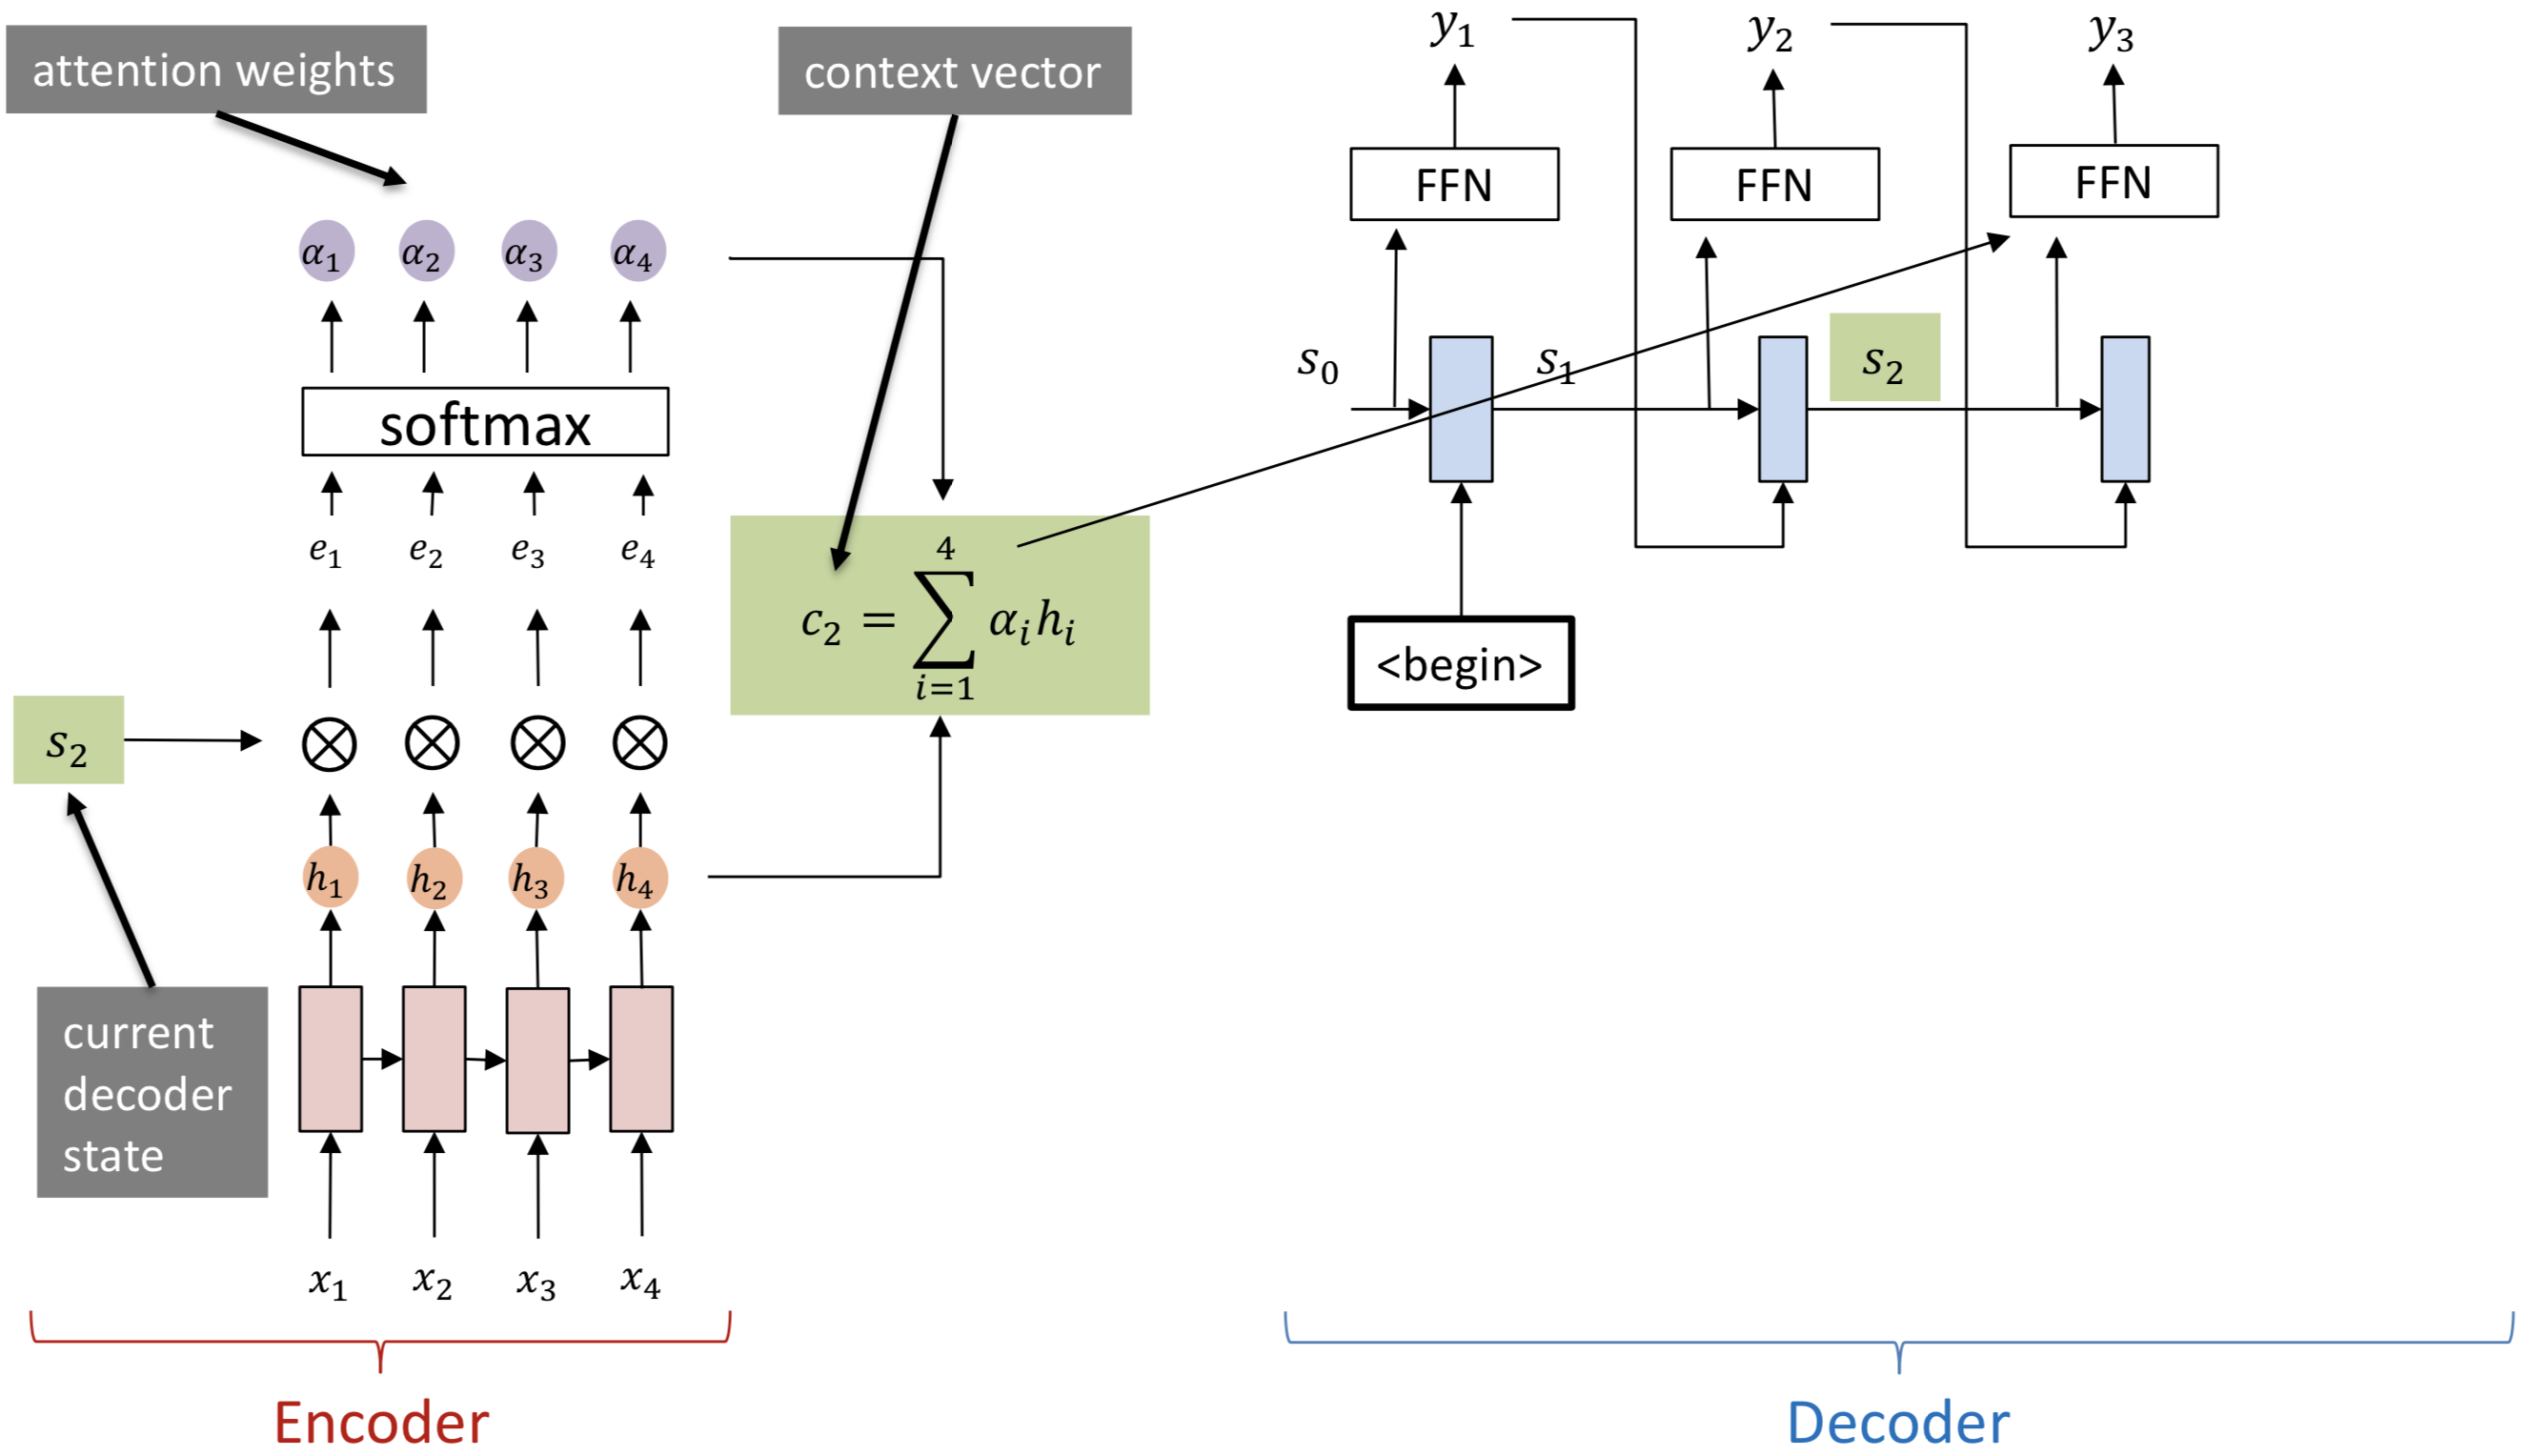
\includegraphics[width=\linewidth]{figures/attention.png}\\
	\textbf{Evaluation von Übersetzung} Es gibt keine Single Source of Truth (mehrere Übersetzungen möglich und korrekt)
	\begin{itemize}
		\item Unigram Precision: $s = \frac{m}{w_t}$, $m$ Wörter die in Ground Truth und Ausgabe auftreten, $w_t$ Länge der Maschinenübersetzung
		\item Bilingual evaluation understudy (BLEU): arbeitet auf n-Grammen (Wortketten), limitiert Anzahl auf Vorkommen in Zielübersetzung, wird gegen mehrere mögliche Übersetzungen evaluiert und Score gemittelt
	\end{itemize}
	\textbf{Transformer} neue neuronale Netzarchitektur auf Basis von Attention ohne RNNs $\rightarrow$ gut parallelisierbar\\
	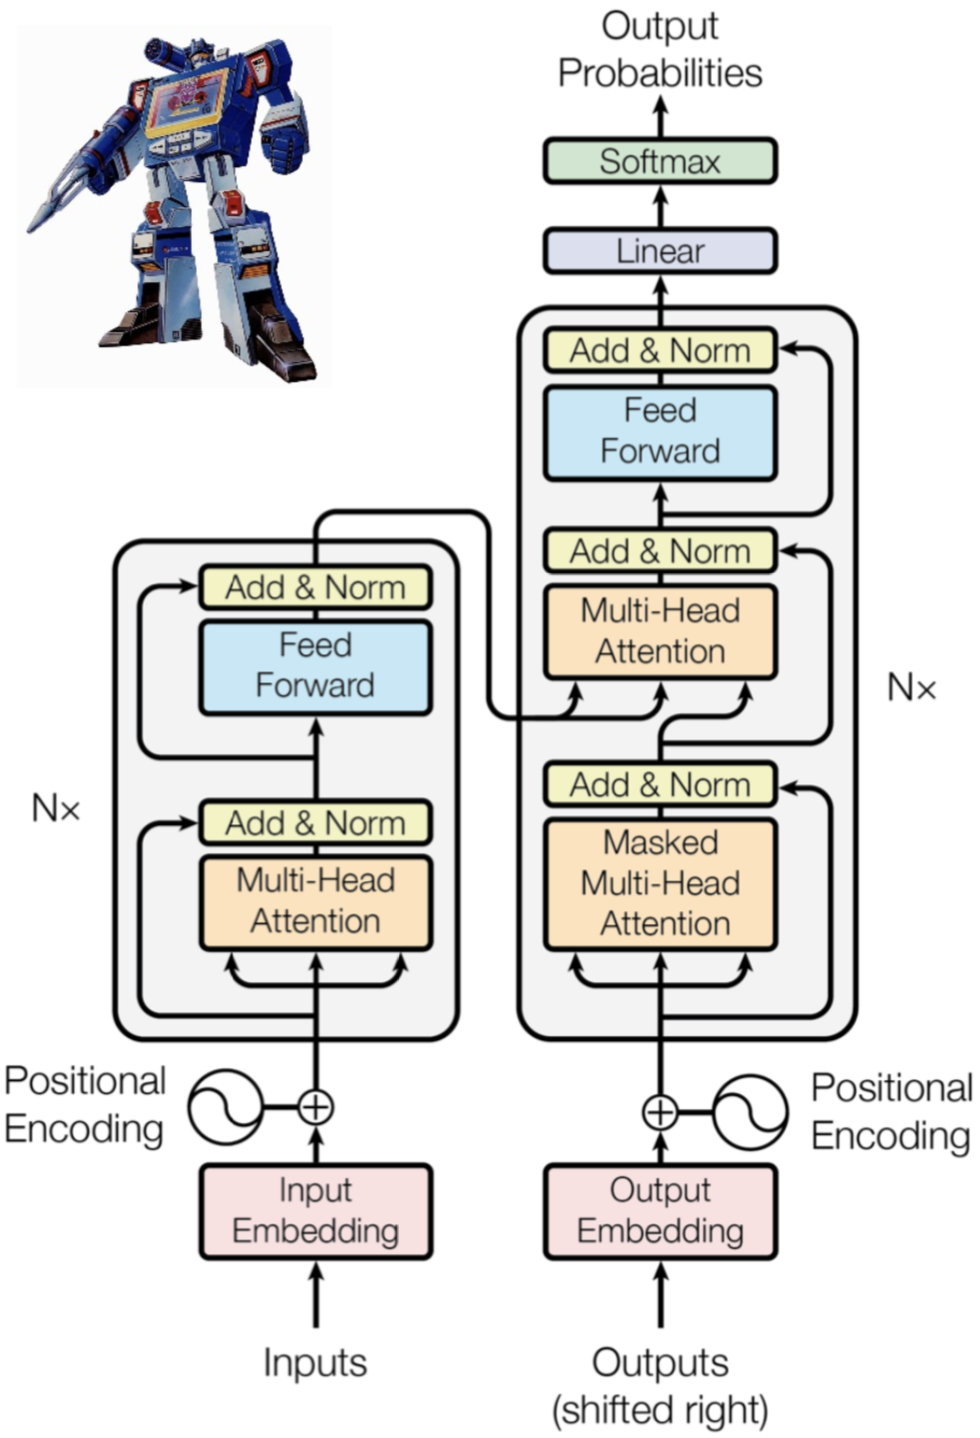
\includegraphics[width=0.5\linewidth]{figures/transformer1.png}
	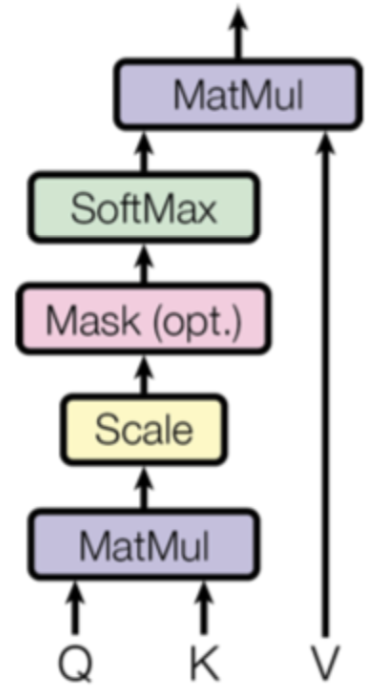
\includegraphics[width=0.5\linewidth]{figures/transformer2.png}
	$$Attention(Q,K,V) = softmax(\frac{QK^T}{\sqrt{d}}) V$$
	$$Q = X \cdot W_1, K = X \cdot W_2, V = X \cdot, W_3$$
	Attention wird komplett aus Input berechnet, es wird eine gewichtete Summe des Inputs erzeugt\\
	\textit{Multihead Attention} Berechne $Q$, $K$, $V$ mehrmals mit unterschiedlichen Gewichtsmatrizen $W_i$, um verschiedenen Fokus zu bekommen.\\
	\textbf{Evolved Transformer} Netzarchitektur wird auch als neuronales Netz mittrainiert.

	% TODO weiter mit Kapitel 8


	% \section{Sequence2Sequence}
	% Abbildung von Sequenzen auf Sequenzen, z.B. bei OCR (Eingabe: Pixelspalten, Ausgabe: Buchstabenklassifikation) oder Spracherkennung. Kann z.B. mit LSTMs umgesetzt werden.\\
	% \textbf{Greedy-Decoder} Ermittelt Klasse durch Maximum auf Ausgabe $\rightarrow$ Entfernen doppelter Zeichen $\rightarrow$ Blanks entfernen\\
	% \textbf{Labellings} Beschreibt die Abbilung der Netzausgabe auf sinnvolle Sequenz.
	% $$B: L'^{T} \rightarrow L^{\leq T}$$
	% $$B(a-ab-) = B(-aa--aabb) = aab$$
	% $$B^{-1}(aab) = {a-ab-, ..., aa-ab, ...}$$
	% Summiere die Wahrscheinlichkeiten aller möglichen Pfade, die zum gewünschten Label führen.\\
	% \textbf{CTC-Loss (Connectionist Temporal Classification)}\\
	% Wird angewendet, wenn die Eingabe eine Zeitsequenz der Länge $T$ ist und als Ausgabe eine unalignierte Labelsequenz der Länge $\leq T$ vorliegt\\
	% 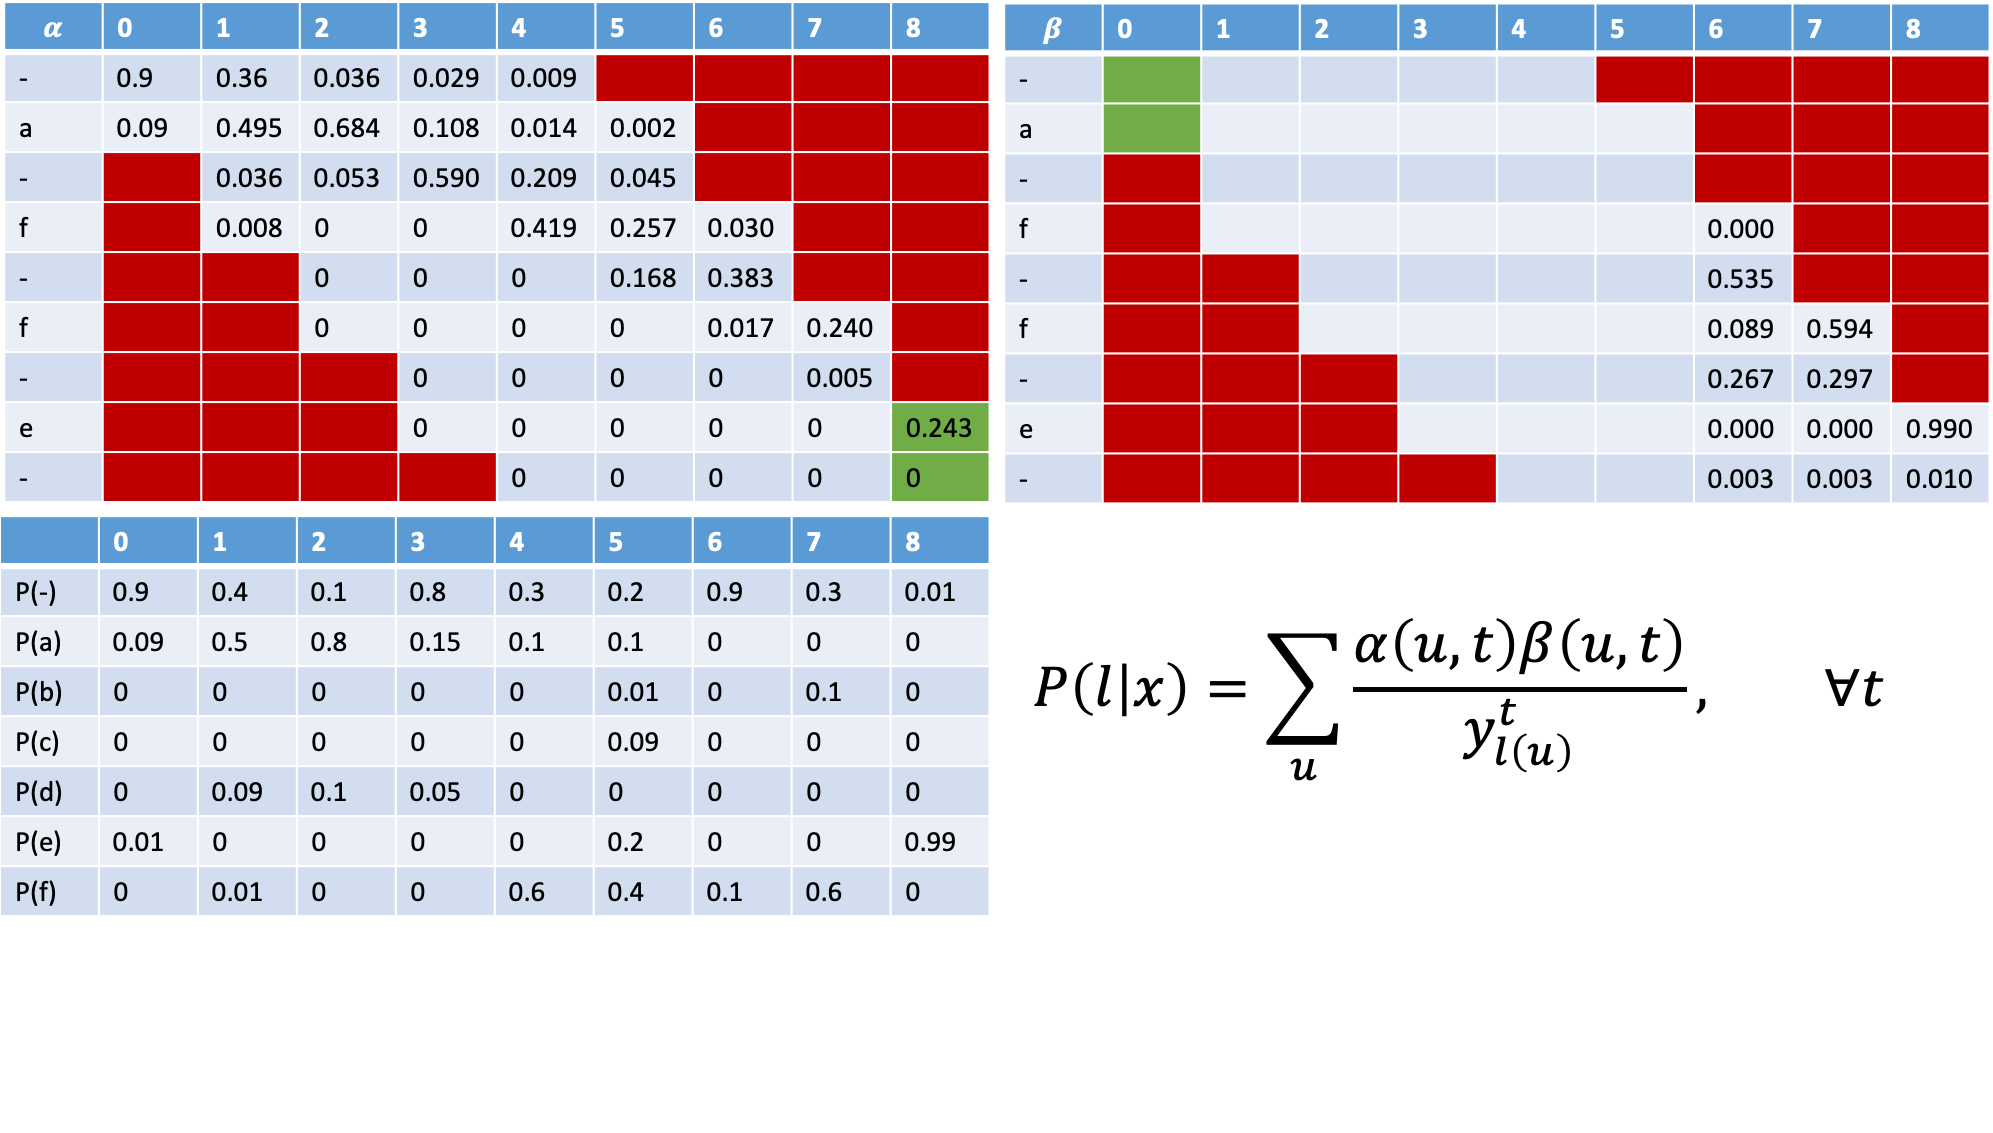
\includegraphics[width=\linewidth]{figures/ctc-algorithmus.png}
	% $$P(l|x) = \sum_{\pi \in B^{-1}(l)} P(\pi|x)$$
	% mit $l$ als gewünschte Sequenz und $x$ als Netzausgabe\\
	% \textit{Loss}: Maximiere $P(l|x)$ bzw. minimiere $-\log(P(l|x))$\\
\end{document}
